%\documentclass{uai2025} % for initial submission
\documentclass[accepted]{uai2025} % after acceptance, for a revised version; 
% also before submission to see how the non-anonymous paper would look like 

%% There is a class option to choose the math font
% \documentclass[mathfont=ptmx]{uai2025} % ptmx math instead of Computer
% Modern (has noticeable issues)
% \documentclass[mathfont=newtx]{uai2025} % newtx fonts (improves upon
% ptmx; less tested, no support)
% NOTE: Only keep *one* line above as appropriate, as it will be replaced
%       automatically for papers to be published. Do not make any other
%       change above this note for an accepted version.

%% Choose your variant of English; be consistent
%\usepackage[american]{babel}
\usepackage[british]{babel}

%% Some suggested packages, as needed:
\usepackage{natbib} % has a nice set of citation styles and commands
\bibliographystyle{plainnat}
\renewcommand{\bibsection}{\subsubsection*{References}}
\usepackage{mathtools} % amsmath with fixes and additions
% \usepackage{siunitx} % for proper typesetting of numbers and units
\usepackage{booktabs} % commands to create good-looking tables
\usepackage{tikz} % nice language for creating drawings and diagrams

%% Provided macros
% \smaller: Because the class footnote size is essentially LaTeX's \small,
%           redefining \footnotesize, we provide the original \footnotesize
%           using this macro.
%           (Use only sparingly, e.g., in drawings, as it is quite small.)


%% Self-defined macros
\newcommand{\swap}[3][-]{#3#1#2} % just an example
\usepackage{soul}
\newcommand{\eop}{{$\blacksquare$}}
\newcommand{\eod}{{${}$\\}}


\newcommand{\cI}{\mathcal{I}}
\newcommand{\A}{\mathcal A}
\newcommand{\anc}{\mathcal A}
\newcommand{\B}{{\mathrm B}}
\newcommand{\bB}{{\mathbb B}}
\newcommand{\cB}{{\mathcal B}}
\newcommand{\bI}{\mathbb{I}}
\newcommand{\R}{{\mathbb R}}
\newcommand{\N}{{\mathbb N}}
%\newcommand{\C}{{\mathbb C}}
\newcommand{\bP}{\mathbb{P}}
\newcommand{\cH}{{\cal H}}
\newcommand{\cA}{{\cal A}}
\newcommand{\cY}{{\cal Y}}
\newcommand{\cW}{{\cal W}}
\newcommand{\cX}{{\cal X}}
\newcommand{\cZ}{{\cal Z}}
\newcommand{\cN}{\mathcal{N}}
\newcommand{\ci}{{\mathfrak C}}
\newcommand{\bE}{\mathbf{E}}
\newcommand{\cS}{\mathcal{S}}
\newcommand{\cT}{\mathcal{T}}
\newcommand{\cM}{{\cal M}}
\newcommand{\cF}{{\cal F}}
\newcommand{\cG}{{\cal G}}
\newcommand{\cC}{{\cal C}}
\newcommand{\cP}{{\cal P}}
\newcommand{\cQ}{{\cal Q}}
\newcommand{\cL}{\mathcal{L}}
\newcommand{\<}{\langle}
\newcommand{\Z}{\mathbb{Z}}
\newcommand{\Ceq}{\stackrel{+}{=}}
\newcommand{\id}{{\bf I}}

\newcommand{\bx}{{\bf x}}
\newcommand{\bX}{{\bf X}}
\newcommand{\bY}{{\bf Y}}
\newcommand{\bZ}{{\bf Z}}
\newcommand{\bN}{{\bf N}}
\newcommand{\bV}{{\bf V}}
\newcommand{\cov}{\operatorname{Cov}}
\newcommand{\var}{\operatorname{Var}}
\newcommand{\dd}{\mathrm{d}}
\newcommand{\bz}{{\bf z}}
\newcommand{\by}{{\bf y}}
\newcommand{\bW}{{\bf W}}
\newcommand{\bC}{{\bf C}}
\newcommand{\An}{{An}}
\newcommand{\Adj}{\operatorname{Adj}}
\newcommand{\PA}{\operatorname{PA}}
\newcommand{\pa}{{pa}}

\newcommand{\MEQ}{\operatorname{MEQ}}
\newcommand{\CI}{\operatorname{CI}}

\newcommand\independent{\protect\mathpalette{\protect\independenT}{\perp}}
\def\independenT#1#2{\mathrel{\rlap{$#1#2$}\mkern2mu{#1#2}}}
\newcommand{\ind}{\independent}

\newcommand{\MD}{\operatorname{MD}}

\usepackage{etoolbox}
%\usepackage{mathabx}

\newtoggle{printcomments}
\toggletrue{printcomments} % Set the flag to true by default.
\togglefalse{printcomments} % Uncomment this to remove all comments in the doc

\newcommand\dominik[1]{%
  \iftoggle{printcomments}{%
    \textcolor{cyan}{Dominik: #1}%
  }{}%
}


\newcommand\philipp[1]{%
  \iftoggle{printcomments}{%
\textcolor{red}{Philipp: #1} % Notes for Leena
  }{}%
}


\newcommand\todo[1]{%
  \iftoggle{printcomments}{%
\textcolor{red}{#1} % Notes for Leena
  }{}%
}


\definecolor{lightgray}{gray}{0.85}
\sethlcolor{Dandelion}

\usetikzlibrary{arrows,shapes,plotmarks,positioning, backgrounds, fit}
\usetikzlibrary{decorations.markings}

\tikzset{>=stealth'} 
\tikzset{node distance=1.5cm}
\tikzstyle{graphnode} = 
   [circle,draw=black,minimum size=22pt,text centered,text
     width=22pt,inner sep=0pt] 
\tikzstyle{var}   =[graphnode,fill=white]
\tikzstyle{vardashed}   =[graphnode,draw=gray,fill=white]
\tikzstyle{obs}   =[graphnode,fill=black,text=white]
\tikzstyle{obsgrey}   =[graphnode,draw=white,fill=lightgray,text=black]
\tikzstyle{par}    =[graphnode,draw=white,fill=red,text=black] 
 \tikzstyle{crucial} =[graphnode,draw=white,fill=yellow,text=black] 
\tikzstyle{fac}   =[rectangle,draw=black,fill=black!25,minimum size=5pt]
\tikzstyle{facprior} =[rectangle,draw=black,fill=black,text=white,minimum size=5pt]
\tikzstyle{edge}  =[draw=white,double=black,very thick,-]
\tikzstyle{blueedge}  =[draw=white,double=blue,very thick,-]
\tikzstyle{rededge}  =[draw=white,double=red,very thick,-]
\tikzstyle{prior} =[rectangle, draw=black, fill=black, minimum size=
5pt, inner sep=0pt]
\tikzstyle{dirprior} = [circle, draw=black, fill=black, minimum
size=5pt, inner sep=0pt]

\tikzstyle{dot_node}=[draw=black,fill=black,shape=circle]

\usepackage{csquotes}
\usepackage{enumitem}
\setlist[itemize]{noitemsep,leftmargin=*,nosep}
\setlist[enumerate]{noitemsep,leftmargin=*,nosep}
\usepackage{cleveref}
\usepackage[standard]{ntheorem}
\newtheorem{assumption}{Assumption}
\usepackage{algorithm}
\usepackage{algorithmic}
\usepackage{subfig}
\definecolor{tabgreen}{HTML}{2ca02c}
\definecolor{tabred}{HTML}{d62728}

\title{On Different Notions of Redundancy in Conditional-Independence-Based Discovery of Graphical Models}
% [Redundancy in Constraint-Based Discovery of Graphical Models]

% The standard author block has changed for UAI 2025 to provide
% more space for long author lists and allow for complex affiliations
%
% All author information is authomatically removed by the class for the
% anonymous submission version of your paper, so you can already add your
% information below.
%
% Add authors
\author[1]{\href{mailto:<philipp.faller@partner.kit.edu>?Subject=Redundancy in Discovery of Graphical Models}{Philipp M. Faller}}{}
\author[2]{Dominik Janzing}
% Add affiliations after the authors
\affil[1]{%
	Karlsruhe Institute of Technology\\
	 Karlsruhe, Germany
}
\affil[2]{%
	Amazon Research\\
	Tübingen, Germany
}
  
\begin{document}
	\maketitle

\begin{abstract}
The goal of conditional-independence-based discovery of graphical models is to find a graph that represents the independence structure of variables in a given dataset.
To learn such a representation, conditional-independence-based approaches conduct a set of statistical tests that suffices to identify the graphical representation under some assumptions on the underlying distribution of the data.
In this work, we highlight that due to the conciseness of the graphical representation, there are often many tests that are not used in the construction of the graph.
These \emph{redundant} tests have the potential to \emph{detect} or sometimes \emph{correct} errors in the learned model.
We show that not all tests contain this additional information and that such redundant tests have to be applied with care.
Precisely, we argue that particularly those conditional (in)dependence statements are interesting that follow only from graphical assumptions but do not hold for every probability distribution.
\end{abstract}

\section{Motivation}
Graphical models have become an indispensable tool for understanding complex systems and making informed decisions in various scientific disciplines \citep{lauritzen1996graphical}. 
They provide insights into the structure within the system and under some additional assumption they  can also be interpreted as \emph{causal models} \citep{pearl2009causality,spirtes2000causation}.

Popular algorithms like PC \citep{spirtes2000causation} or SP \citep{raskutti2018learning} utilise (conditional) independence statements to infer the graphical structure.
However, a key challenge arises from the statistical hardness of conditional independence (CI) tests. 
As highlighted by \citet{shah2020hardness}, CI-tests cannot have valid false positive control and power against arbitrary alternatives at the same time. \todo{double check if this is what the paper says}
Additionally, constraint-based algorithms often rely on assumptions like \emph{faithfulness}, which means that the graphical structure does not only imply \emph{in}dependences but also dependences.
\citet{uhler2013geometry} showed that this assumption can be problematic in the finite-sample regime since even faithful distributions can be close enough to unfaithful ones for a CI-test to fail.
It is also probably violated in domains where systems evolve to equilibrium states, as in many biological settings \citep{andersen2013expect}.
On the other hand, even a single wrong result of a CI-test can result in arbitrarily large changes in the resulting graphical model (as e.g. in \cref{ex:wrong_v_structure}).
%This is especially worrisome if the graphical model is interpreted as a causal model.


In the worst case, conditional-independence-based discovery of graphical models requires exponentially many CI-tests in the number of nodes \citep{korhonen2024structural,zhang2024membership}.
%TODO write better. THis makes it sound as if our idea is trivial
Despite the large number of required tests, the set of possible graphical models can still be small compared to the set of possible independence models.
% as \cite{janzing2023reinterpreting} have highlighted.
%They show that in fact the independence structures implied by graphical models are indeed a set of finite VC dimension in the learning scenario they formalize.
While e.g. \citet{shiragur2024causal} proposed a method to reduce the number of required test (while sacrificing details of the models),
in this paper we will advocate to use additional CI-tests to evaluate the graphs, which has been proposed implicitly or explicitly before  \citep{textor2016robust,eulig2023toward,janzing2023reinterpreting}.
In spirit, this follows \citet{raskutti2018learning}, who have hypothesised that there exists a statistical/computational trade-off for causal discovery. 
We will argue that not all CI-tests carry additional information (and can therefore be used to evaluate a graphical model), but only those tests for which the result follows from \emph{graphical} restrictions instead of the laws of probability.

\begin{example}[Non-Generic Collider]
\label{ex:motivation}
	Consider a probability distribution that is Markovian and faithful to the graph $X_1\to Y\leftarrow X_2$ for random variables $X_1, X_2, Y$.
	Suppose we use the PC algorithm to recover the graph.
	The algorithm will conduct all pairwise marginal independence tests.
	These tests already identify the given DAG.
    But clearly, the graph also entails $X_1\not\ind X_2\mid Y$  under the faithfulness assumption.
    %\footnote{In fact, this already follows e.g. from the weaker \emph{orientation faithfulness} \cite{ramsey2006adjacency}}
	On the other hand, this dependence does not follow for all probability distributions,
    %as we will prove later in \cref{prop:sufficient_cond_non_graphoid}.
    as we will see by constructing a counterexample. 
    We will use similar constructions multiple times.
	Assume\footnote{%If the reader is uncomfortable with the vector-valued random variable $Y$, 
    One could also think about a variable $Y$ taking values in the natural numbers where $X_1$ and $X_2$ only depend on disjoint sets of bits in the binary expansion of $Y$.} $Y=(Y_1, Y_2)\in \R^2$. Now assume $Y_1$ only depends on $X_1$ and $Y_2$ only on $X_2$ as in \cref{fig:three_v_structures}.
	Then we would get the same marginal (in)dependences as before, but not the conditional dependence from above.
     On the other hand, if we have $X_1\not\ind Y$ and $X_1\ind X_2$ we also have $X_1
    \not\ind Y\mid X_2$ for all probability distribution.
    This follows from the Graphoid axioms, described later in \cref{def:graphoid}.
\begin{figure}[htp]
\centering
    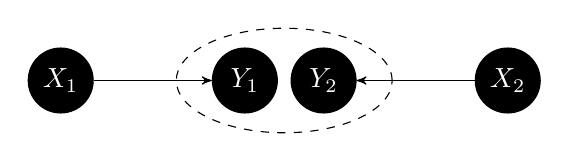
\begin{tikzpicture}
	% Original nodes
	\node[obs] (A) {$X_1$};
	\node[obs, right=of A] (B1) {$Y_1$};
	\node[obs, right=of A, xshift=1cm] (B2) {$Y_2$};
	
	% Circle enclosing B1 and B2
	\begin{scope}[on background layer]
		\node[draw, ellipse, dashed, fit=(B1) (B2), inner sep=0.05cm] (B_group) {};
	\end{scope}
	
	\node[obs, right=of B2] (C) {$X_2$} edge[->] (B2);
	%\node[obs, below =of B_group] (D) {$D$} edge[<-] (B2);
	%\node[vardashed, below=of A] (L1) {$L_1$} edge[->] (A) edge[->] (D);
	%\node[vardashed, below=of C] (L2) {$L_2$} edge[->] (C) edge[->] (D);
	
	% Connection from A to B1 and B2
	\draw[->] (A) -- (B1);
	%\draw[->] (B1) -- (D);
	
	
	% Add a label for the group
	%\node[below=0.1cm of B_group.south] {$B$};
\end{tikzpicture}
	\caption{The marginal independence tests identify the faithful DAG (with $Y$ as single variable). But the collider structure $X_1-Y-X_2$ implies $X_1\not\ind X_2 \mid Y$ for all \emph{faithful} distributions. This does not hold for every distribution. On the contrary, given the marginal tests we have e.g. $X_1\not \ind Y\mid X_2$ for all distributions.}
	\label{fig:three_v_structures}
\end{figure}

	
In other words there is a dependence that follows from the assumption that the underlying distribution can be represented by a \emph{faithful} DAG, but the dependence does not hold for all distributions.
At the same time there are CI-tests that carry no additional information.
\end{example}

\subsection{Contributions}
This paper aims to provide a novel perspective on CI-based discovery of graphical models.
Precisely,
\begin{itemize}
	\item we propose two notions of redundancy of CI-statements: the ones that already follow for all distributions and the ones that are only implied by graphical assumptions,
	\item we show theoretically and experimentally that the former can give a misleading impression of evidence for a graphical model, % and often only the latter can falsify a graphical model,
	\item we exemplify how these insights can be used to \emph{detect} and \emph{correct} errors in conditional independence tests
	\item we highlight how our novel perspective generalises previous results on robustness of graph discovery.
\end{itemize}
%There are known observations in the same spirit (e.g. \citet{ramsey2006adjacency,colombo2014order,raskutti2018learning}).
To the best of our knowledge, we are the first to systematically investigate the redundancy of CI-statements.
This work aims to contribute to the discussion on how graphical models should be evaluated and to question which empirical observations are actual evidence and therefore capable of corroborating a model.

\section{Redundancy of CIs}
\paragraph{Notation}
We will now introduce some notation and basic concepts.
For more detailed definitions, we refer the reader to \cref{sec:further_definitions}.
We denote a random variable with upper case letter $X$. 
A set of random variables is denoted with bold face letters $\bX$.
Let $\bV$ be a finite set variables.
An independence model $M$ over $\bV$ is a set of triplets $\bX, \bY, \bZ\subseteq \bV$ where $\bX\neq\emptyset \neq\bY$ and $\bX, \bY, \bZ$ are disjoint.
Then we say $\bX$ is \emph{independent} from $\bY$ given $\bZ$ and write $\bX\ind_{\mspace{-8mu} M}\bY\mid \bZ$, where we often omit the subscript.
If $(\bX, \bY, \bZ) \not\in M$ we say they are dependent and write  $\bX\not\ind_{\mspace{-8mu} M}\bY\mid \bZ$.
A \emph{CI-statement} is a quadruple of $\bX, \bY, \bZ$ and a boolean value, indicating whether the independence holds.
For a set of CI-statements $L$ we slightly abuse notation and write $L\subseteq M$ if for $(\bX, \bY, \bZ, b)\in L$ we have $b=((\bX,\bY,\bZ)\in M$).
We also sometimes write a CI-statement as function $\CI: \bX, \bY, \bZ\mapsto b$ or $\bX \ind \bY\mid \bZ$ if $(\bX, \bY, \bZ)\in M$ and $\bX \not\ind \bY\mid \bZ$ if $(\bX, \bY, \bZ)\not\in M$.
Note that with \emph{in}dependences we refer to statements of the form $\bX\ind \bY\mid \bZ$ and with dependences to $\bX\not\ind \bY\mid \bZ$, while with CI-statement we refer to both of them.
A probability distribution over $\bV$ induces an independence model via probabilistic conditional independence.
Graphical models can also be used to represent independence models and we denote a model induced by a graph $G$ as $M_G$.
For an undirected graph $G$ we define $(\bX, \bY, \bZ) \in M_G$ iff $\bX$ is separated from $\bY$ given $\bZ$.
For DAGs $(\bX, \bY, \bZ) \in M_G$ iff $\bX$ is $d$-separated from $\bY$ given $\bZ$.
In both cases we also write $\bX\perp_G \bY\mid \bZ$.
By \emph{graphical model} we refer to \emph{either} an undirected graph or a DAG (and its respective independence model).\footnote{We restrict our attention to undirected graphs and DAGs.
But our insights can be applied to any model that is equipped with a notion of independence between nodes, such as chain graphs \citep{lauritzen1996graphical}, completed partial DAGs, maximal ancestral graphs, partial ancestral graphs \citep{spirtes2000causation} or acyclic directed mixed graphs \citep{richardson2003markov}.}
A graph is \emph{Markovian} to an independence model $M$ if $(\bX, \bY, \bZ) \in M_G \implies(\bX, \bY, \bZ) \in M$ and it is \emph{faithful} if $(\bX, \bY, \bZ) \in M \implies (\bX, \bY, \bZ) \in M_G$.
Again, we slightly abuse notation and say $G$ is Markovian to a set of CI-statements $L$ when all \emph{in}dependences in $G$ are contained and true in $L$.
As a convenient shorthand we also use 
%\begin{displaymath}
 $   \CI(\bV) := \{(X, Y, \bZ) :\: X, Y\in \bV,\, \bZ\subseteq \bV\setminus\{X, Y\},\, X\neq Y\}$.
%\end{displaymath}
For independence models $M, M'$ over $\bV$ we define the \emph{Markov distance} w.r.t. $S\subseteq \CI(V)$ via
%\begin{displaymath}
 $   \MD_S(M, M') = \sum_{s\in S} \mathbb{I}\left[(s\in M) \neq (s\in M')\right]$.
%\end{displaymath}
We omit the subscript if $S=\CI(\bV)$.
In this case, \citet{wahl2024metrics} call this \emph{s/c-metric} and show that it is a proper metric.
We extend the definition to graphs by considering their induced independence model.

\subsection{Graphs as error correcting codes}
\label{subsec:noisy_channel}
\todo{Section even necessary?}
\looseness=-1To motivate why we call some conditional independence tests \enquote{redundant}, we will phrase graph discovery as a coding problem.
Suppose a sender picks a graph $G$ from a set of graphs. %$\cG$ of all graphs with $n\in\N$ nodes.
Since the Markov-equivalence class of this graph is identified by a sequence of CI-statements, she can encode this equivalence class in a binary string $s\in \{0, 1\}^k$ for some $k\in \N$, where each bit represents whether a certain CI-statement holds or not.
If a receiver knows the sequence of CI-statements, she can perfectly recover the equivalence class of $G$ from $s$.
In this scenario the mapping $G\mapsto s$ is a coding scheme.
Then a (deterministic) CI-based discovery algorithm implicitly defines a decoding scheme $s \mapsto G$.
Unfortunately, the discovery algorithm rarely receives $s$, but a noisy version of it, since the CI-tests can have errornous outputs.
If we assume, for now, that the errors of each bit are independent, Shannon's noisy-channel coding theorem \citep{mackay2003information} asserts that there is a coding scheme 
%with rate $R\in \R$ 
such that messages can be transmitted with arbitrarily small error probability as the number of sent bits approaches infinity.\footnote{It is worth noting that the relationship to the noisy-channel coding theorem is just an analogy and the theorem cannot be applied to our setting. 
The reason is that the theorem holds when the number of sent bits approaches infinity while we can only conduct finitely many CI-tests.}
%, where $R$ quantifies how much information each bit of $s$ contains.
This begs the question what it would mean to have these \emph{redundant} bits added to $s$.
In a (literal) noisy channel one could resend bits, but clearly redoing a CI-test does not give us additional information. 
%(as the \enquote{channel} applies exactly the same noise to the result).
Also techniques like bootstrapping cannot help if the errors come from faithfulness violations.
%The theorem only guarantees the existence of such a coding scheme.
%But since in the scheme described above the rate can be decreased by adding \emph{redundant} independence tests to the messages, we will call conditional independence tests that contain no additional information about the identity of $G$ redundant.
In the rest of this work we will discuss which tests are suitable to add redundancy to our encoding.
%\dominik{not clear whether there exists enough tests to enable reliable information transmission (of course depends on the error rate)}


%Maybe present Shannon as lower bound for amount of redundancy if additional tests are supposed to help.
%Then say that tests can be dependent, which is why we look at graphoids next.

\subsection{Graphs, Graphoids and Redundancy}
The central observation of this paper is that a graphical model usually entails more CI-statements than the ones necessary to identify their Markov-equivalence class, as we have already seen in  \cref{ex:motivation}.
In other words, the space of independence models entailed by a graphical model is typically smaller than the space of all possible independence models.
These tests are our candidates to be used for error detection and correction, which motivates the following definition.

\begin{definition}[Graphical-Redundancy]
	\label{def:graphical_redundancy}
	Let $L$ be a set of CI-statements  and $s\not\in L$ be another CI-statement.
	Let $\cG$ be a set of graphical models and $\cM_\cG$ the set of respective independence models.
	We call $s$ \emph{graphically-redundant} w.r.t. $\cM_\cG$ if $\{s\}\subseteq M_G$ whenever $L\subseteq M_G$ for any graph $G\in \cG$.
	%If $\cG$ is the set of DAGs we call $s$ \emph{DAG-redundant.} 
\end{definition}
\todo{In camera-ready write out wrt.}
Note, that this definition is w.r.t. a set of (previous) CI-tests \emph{and} a class of graphical models.
The former depends on the specific algorithm used for discovery, while the latter depends on the assumptions that we make on the data.

\label{subsec:redundancy}
%Show Graphoid axioms, say they are not complete, show how Graphical models reduce space of possible independences\\

\looseness=-1In the noisy-channel model in \cref{subsec:noisy_channel} we have assumed that bit errors occur independently.
But it is well-known that the output of CI-tests on the same dataset can be dependent.
Especially, there are cases where some (in)dependence statements follow from a set of (in)dependence statements for \emph{all} probability distributions.
\citet{pearl2022graphoids} have provided a sound set of logical rules to derive independences:
\begin{definition}[Graphoid Axioms]
	\label{def:graphoid}
	Let $M$ be an independence model over variables $\bV$ and $\bX, \bY, \bZ, \bW\subseteq \bV$ be disjoint with $\bX\neq\emptyset\neq \bY$. We call $M$ a \emph{semi-graphoid} if 
	\begin{enumerate}
		\item $\bX\ind \bY\mid \bZ \iff \bY\ind \bX\mid  \bZ$
		\item $\bX\ind  \bY\cup \bW \mid \bZ \implies \bX \ind \bY \mid\bZ \ \land\  \bX \ind \bW \mid \bZ$
		\item $\bX\ind \bY\cup \bW \mid \bZ \\ \implies \bX\ind  \bY \mid\bZ\cup \bW\ \land\  \bX\ind\bW \mid \bZ\cup \bY$
		\item $\bX\ind\bY \mid \bZ \ \land\  \bX \ind\bW \mid \bZ\cup \bY \implies \bX\ind\bY\cup \bW \mid \bZ $
	\end{enumerate}
	$M$ is called \emph{graphoid} if further holds
	\begin{enumerate}[resume]
		\item $\bX\ind\bY \mid \bZ\cup \bW \ \land\  \bX\ind\bW\mid \bZ\cup \bY \\\implies \bX\ind\bY\cup \bW\mid \bZ$.
	\end{enumerate}
\end{definition}
The independence model of a probability distribution is a semi-Graphoid and it is a Graphoid  if the distribution is positive \citep{lauritzen1996graphical}.
Although these rules are sound, they are not complete and there cannot be a finite, sound and complete set of axioms to describe conditional independence in probability distributions \citep{studeny1992conditional}.

Since the semi-Graphoid rules hold for every distribution, they obviously also hold for every empirical distribution.
Moreover, the following proposition shows that for partial correlations these rules have a certain continuity property.

\begin{proposition}[Continuity of Correlational Graphoid]
	\label{prop:continuity_partial_corr}
	Let $X, Y, Z$ be real-valued random variables and $\epsilon > 0$.
	Then
	\begin{enumerate}
		\item $|\rho_{X,Y\cdot Z}| \le \epsilon \iff |\rho_{Y,X\cdot Z}|\le \epsilon$
		\item $|\rho_{X,Y\cup W\cdot Z}| \le \epsilon \implies  |\rho_{X,Y\cdot Z}| \le \epsilon \ \land\  |\rho_{X,W\cdot Z}| \le \epsilon$
		\item $|\rho_{X,Y\cup W\cdot Z}| \le \epsilon \le 1/2 \\ \implies |\rho_{X,Y\cdot Z\cup W} |\le 2\epsilon \ \land\  |\rho_{X,W\cdot Z\cup Y}| \le 2\epsilon$
		\item $|\rho_{X,Y\cdot Z}| \le \epsilon \ \land\  |\rho_{X,W\cdot Z\cup Y}| \le \epsilon \\ \implies |\rho_{X,Y\cup W\cdot Z}| \le 2\epsilon$
	\end{enumerate} 
	If we further assume $ \rho_{W,Y\cdot Z} \le 1 - \epsilon$ we get
	\begin{enumerate}[resume]
		\item $|\rho_{X,Y\cdot Z\cup W}| \le \epsilon \le 1/2 \ \land\  |\rho_{X,W\cdot Z\cup Y}| \le \epsilon \le 1/2\\\implies  |\rho_{X,Y\cup W\cdot Z}| \le 4\epsilon$.
	\end{enumerate}
\end{proposition}
All proofs are in \cref{sec:proofs}. 
This means that even if some CI-statements hold only approximately, they are likely to influence other test results according to the Graphoid axioms.
In the analogy to the noisy-channel model from \cref{subsec:noisy_channel} this would mean that these tests do not contain redundant information.
Therefore, we want to differentiate between tests that are implied by the graphical structure alone and tests that already follow for all probability distributions.
\begin{definition}[Probabilistic-Redundancy]
	\label{def:prob_redundant}
	Let $L$ be a set of CI-statements  and $s\not\in L$ be another CI statement.
	We call $s$ \emph{probabilistically-redundant} if $\{s\}\subseteq M$ for any independence model induced by a probability distribution with $L\subseteq M$. 
\end{definition}
Although the CI-statements we are interested in are the ones that are not probabilistically redundant, it is potentially hard to operationalise this definition.
Due to the aforementioned incompleteness of any finite system of axioms for probabilitic conditional independence, we will instead consider all CI-statements that follow via the Graphoid axioms.
\begin{definition}[Graphoid-Redundancy]
	\label{def:graphoid_redundancy}
	Let $L$ be a set of CI-statements  and $s\not\in L$ be another CI statement.
	We call $s$ \emph{Graphoid-redundant} if $\{s\}\subseteq M$ for any Graphoid independence model with $L\subseteq M$. 
\end{definition}
Since the Graphoid axioms are sound, Graphoid-redundancy\footnote{For simplicity, we do not further differentiate between semi-Graphoid-redundant and Graphoid-redundant CI-statements.} is a sufficient criterion for a CI-statement to also be probabilistically redundant.
For a set $L$ of CI-statements we denote with $C(L)$ the \emph{Graphoid-closure} of $L$, i.e. the set of all CI-statements that can be derived from $L$ by finitely many applications of the rules in \cref{def:graphoid}.
%Clearly, conducting additional, Graphoid-redundant tests does not give us additional evidence for or against a certain graphical model given a known set $L$, as the result is already implied (with high probability) by $L$. 
%And as every non-negative distribution is a Graphoid, 
The following definition captures the CI-statements where the results are not already implied by the Graphoid axioms but follow solely from graphical assumptions.
\begin{definition}[Purely Graphical Redundancy]
	\label{def:purely_graphical_red}
	Let $L$ be a set of CI statements  and $s\not\in L$ be another CI statement.
	We call $s$ \emph{purely graphically redundant} if $s$ is graphically redundant but not graphoid redundant. 
\end{definition}
%Note, that every Graphoid-redundant test is also graphically redundant (for the graphical model we consider).
This definition begs the question whether there is a criterion to find the purely graphically redundant CI-statements.
We will first present results from the literature showing which CI-statements cannot be purely graphically redundant and then see a sufficient graphical criterion that covers a broad class of examples where they are.
Especially, \cref{prop:markov_network_markovian,prop:protocol_graph_markovian} show cases where all \emph{in}dependences are Graphoid redundant.
%\todo{Explicitly say that CI-statemnt is either ind or dep and independence and dependence is explicit.}
\begin{theorem}[\citet{verma1990causal} Theorem 2]
	\label{prop:protocol_graph_markovian}
	Let $M$ be a Graphoid independence model over a set of nodes $\bV$, and $\pi:\bV\to \N$ be an ordering of $\bV$.
	Let $L_\pi$ be a causal input list for $M$, i.e.  for $X, Y, \bZ \in \CI(\bV)$ we have $\CI(X, Y\mid \bZ) \in L_\pi$ iff
	\begin{displaymath}
		\pi(X) < \pi(Y)\  \land\  \forall Z\in\bZ :\: \pi(X) \neq \pi(Z) < \pi(Y). \todo{Insert space for readability}
	\end{displaymath}
	Let $G_\pi$ be the DAG over $V$ with an edge from $X\in\bV$ to $Y\in \bV$ iff $(X\not\ind Y \mid \bZ) \in L_\pi$ for some $\bZ\subseteq \bV$.
	Then $G_\pi$ is Markovian to $C(L_\pi)$.
\end{theorem}
\todo{Write sentence on relevance of theorem.}
\begin{theorem}[\citet{geiger1993logical} Theorem 12]
	\label{prop:markov_network_markovian}
	Let $M$ be a Graphoid independence model over a set of nodes $\bV$.
	Let $L$ be the set of CI-statements
	\begin{displaymath}
		L = \{\CI(X, Y\,|\, \bV\setminus\{X, Y\}) :\: X, Y\in \bV,\, X\neq Y\}.
	\end{displaymath}
	Let $G_L$ be the undirected graph over $\bV$ with an edge between $X, Y\in \bV$ iff $(X\not\ind Y \mid \bV\setminus\{X, Y\}) \in L$.
	Then $G_L$ is Markovian to $C(L)$.
\end{theorem}
A similar result has been shown by \citet{studeny1998chain} for chain graphs. 
%So for the procedures described in these theorems no \emph{in}dependence can be purely graphically redundant.
Note, that the PC algorithm is not guaranteed to return Markovian results (see \cref{ex:pc_not_markov}).

No graph discovery algorithm can rely on the Markov assumption alone.
Most of them also use the faithfulness assumption. 
The latter is especially troublesome as there are many applications where it may be violated, as we have mentioned before.
\dominik{do we have references there?}
But in the cases above, none of the \emph{in}dependence statements can be used as additional redundancy.
So here, it is only due to faithfulness (and similar assumptions) that we can have purely graphical redundancy at all.
But also not all of the dependences are good candidates for error detection and correction.
As \citet{bouckaert1995bayesian} shows, there are also dependences that follow from the Graphoid axioms as their contrapositives.
\begin{definition}[Coupling]
    Let $G$ be an undirected graph over $\bV$ and $\bX, \bY, \bZ \subseteq \bV$ be disjoint with $\bX\neq\emptyset\neq\bY$.
    Then $\bX$ and $\bY$ are \emph{coupled} given $\bZ$ if there are $X\in \bX, Y\in \bY$ or $Y\in \bX, X\in\bY$ such that
    \begin{itemize}
        \item $(X-Y)\in G$
        \item $\Adj(X)\subset \bX\cup\bY\cup\bZ$
    \end{itemize}
	Now let $G$ be a DAG. Then
    $\bX$ and $\bY$ are \emph{coupled} given $\bZ$ if there are $X\in \bX, Y\in \bY$ or $Y\in \bX, X\in\bY$ such that
    \begin{itemize}
        \item $(X\to Y)\in G$
        \item $\PA(Y)\subset \bX\cup\bY\cup\bZ$
        \item $\exists \mathbf{Q} \subseteq \bX\cup\bY\cup\bZ\setminus\{X, Y\}$ s.t. $\bZ\subseteq \mathbf{Q}$ and \\$X\perp_{G-(X\to Y)} Y\mid \mathbf{Q}$.
    \end{itemize}
\end{definition}
\citet{bouckaert1995bayesian} show that this graphical criterion gives dependence statements that follow for all Graphoid models.
\begin{theorem}[\citet{bouckaert1995bayesian} Theorem 3.6 and 3.10]
	\label{prop:coupling}
    Let $M$ be a Graphoid independence model over $\bV$ and $G$ be a graph that is Markovian to $M$.
    Let $\bX, \bY, \bZ
    \subseteq \bV$.
    If $\bX, \bY, \bZ$ are  coupled in $G$, then $\bX\not\ind_{\mspace{-8mu}M}\bY\mid \bZ$.
\end{theorem}
So this holds especially in the graphs from \cref{prop:markov_network_markovian,prop:protocol_graph_markovian}.
On the other hand, we can  characterise conditions under which a given dependency statement is guaranteed to be purely graphically redundant.
So whenever a graphical model implies such a dependency we can utilise it as additional redundancy.
First, we introduce some notation:
let  $(X, Y, \bZ), (A, B, \bC) \in \CI(\bV)$, $G$ be a graphical model over $\bV$ and $s = (X\not\ind Y \mid \bZ)$. \todo{Strictly, it would be better to have $s:=(X, Y\bZ).$}
We say a path $(A, \dots, B)$ is $s$-active given $\bC$ if it is active given $\bC$ w.r.t. the respective graphical separation and there is no sub-path $(X, \dots, Y)$ that is active given $\bZ$.
Then we write $A\perp_G^{s} B\mid \bC$ iff there are no $s$-active paths between $A$ and $B$ given $\bC$.
\begin{proposition}
	\label{prop:sufficient_cond_non_graphoid}
	Let $L$ be a set of CI-statements and $s:=(X\not\ind Y\mid \bZ)\not\in L$ for some $(X, Y, \bZ) \in \CI(\bV)$.
	Let $G$ be a graphical model over $\bV$ such that $G$ is Markovian to $C(L)$ and $X\not\perp_{G} Y\mid \bZ$.
	If there are no $(A, B, \bC) \in \CI(\bV)$ such that $(A
	\not\ind B\mid \bC) \in L$ and $A\perp_{G}^s B\mid \bC$, then $s$ is purely graphically redundant given $L$.
\end{proposition}


\todo{Remove? 
\begin{remark}
Given that the purely graphically redundant tests depend on the ground truth graphical model, one might wonder whether one can define a \emph{condition number} of a graph in analogy to the condition number of a matrix, where the numerical stability of matrix inversion depends on the matrix itself. But clearly here things are even more involved as also the given CI-statements (i.e. the discovery algorithm that already conducted tests) is relevant.
\end{remark}}

\todo{Necessary?}
%In the following we will apply these results in order to \emph{detect} and \emph{correct} errors, in analogy to coding theory.
\todo{Put back in bridge sentence?}
%For each of these tasks, we highlight examples for two cases of graphical model assumptions. 
%The former is primarily an illustrative example, although the results might be of interest on their own.
\section{Error Detection and Correction}
\label{sec:error_detection_correction}

%Previously we have seen that Graphoid redundant CI-statements contain little additional information and how we can spot purely graphically redundant statements. 
Since Graphoid-redundant tests are unlikely to contradict the given tests, they might give the misleading impression of evidence for a model.
In the following we will \emph{detect} and \emph{correct} errors with purely graphically redundant tests.
\todo{Put back sentence to end of previous section?}
\subsection{Error Detection}

In the beginning of this section we will focus on spanning trees (c.f. \cref{sec:further_definitions}) for two reasons. First, they are a simple class of examples. But also, as we will see, they impose particularly strong graphical assumptions.

\paragraph{Error Detection in Spanning Trees}
  %, i.e. the set of graphs %with $n$ nodes 
% such that every pair of nodes is connected by exactly one path.
%We will omit $n$ in the following.
%Let $P$ be a distribution that is Markovian and faithful to some $T\in\cT$.

%Since we have seen in \cref{prop:continuity_partial_corr} that graphoid-redundant tests are of little interest if we want to detect errors, we will only consider a subset of possible CI-tests in the following section.
%The particularly strong restrictions of a spanning tree allow us to ignore many possible tests and still achieve identifiability.
%Moreover, we can also still get purely graphical redundancy.
%An example that is too simple to achieve this is the following modification of the Chow-Liu-Algorithm \cite{chow1968approximating}.
\looseness=-1Suppose we use the CI-statements from \cref{prop:markov_network_markovian} to find an undirected graph.
Although this approach is quite efficient algorithmically, it is sensitive to errors.
Each of the conducted CI-tests directly corresponds to the presence or absence of an edge.
In other words, a single error already makes it impossible to find the correct graph.
But, in this case \cref{prop:sufficient_cond_non_graphoid} equips us with plenty of CI-statements that could be used to falsify the result under the faithfulness assumption.
\begin{example}[Transitive Dependence]
\label{ex:transitive_dependence}
    \looseness=-1Consider the independence model that is Markov and faithful to the graph in \cref{fig:transitive_dependence}.
    Let $L$ be the set of CI-statements from \cref{prop:markov_network_markovian}.
    Let $i,j\in\N$ such that the nodes $X_i$ and $X_j$ are not connected by an edge.
    By construction, $L$ does not contain a dependence statement involving $X_i$ and $X_j$.
    So especially, $L$ does not contain a dependence between nodes $X_k$ and $X_l$ with $k, l\in\N$ such that $X_k$ and $X_l$ are only connected over a non-trivial path.
    So by \cref{prop:sufficient_cond_non_graphoid}, every dependence between non-adjacent nodes is purely graphically redundant.\footnote{In practice, especially the dependences over short paths are of interest. As the data processing inequality \citep{mackay2003information} bounds the mutual information along a path, the dependences become increasingly weaker the longer a (non-deterministic) path is. %(unless all links are deterministic).
    }
    By \cref{prop:markov_network_markovian} all \emph{in}dependences are Graphoid redundant.
    \begin{figure}[htp]
		\centering
		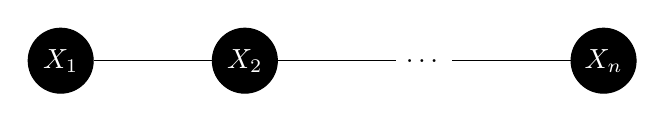
\begin{tikzpicture}
			\node[obs] (X1) {$X_1$} ;
			\node[obs, right=of X1] (X2) {$X_2$} edge[-] (X1) ;
            \node[right=of X2] (X3) {$\dots$} edge[-] (X2) ;
            \node[obs, right=of X3] (Xn) {$X_n$} edge[-] (X3) ;
			
		\end{tikzpicture}
		\caption{In this graph, every dependence along more than one edge is purely graphically redundant given the CI-statements from \cref{prop:markov_network_markovian}.}
		\label{fig:transitive_dependence}
	\end{figure}
\end{example}
The next example shows that the purely graphically redundant statements are imposed by \emph{strong} graphical assumptions.
\begin{example}[Implied Connectedness]
\label{ex:implied_connectedness}
    Suppose again our independence model is Markovian and faithful to the graph in \cref{fig:transitive_dependence}.
    Now suppose we have a set \begin{displaymath}
        L = \{(X_i\ind X_n \,|\, \bV\setminus\{X_i, X_n\}) :\: i \in \{1, \dots, n-2\}\}.
    \end{displaymath}
    If we assume that the independence model is Markovian and faithful to a spanning tree, the statement $X_{n-1} \not\ind X_n\mid \bV\setminus\{X_{n-1}, X_n\}$ is graphically redundant, as otherwise $X_n$ would be disconnected from the graph.
    According to \cref{prop:sufficient_cond_non_graphoid} it is even purely graphically redundant.
    But if we only assume the underlying graph is any undirected graph, this would not follow.
    In terms of error detection this means that a test with result $X_{n-1}\ind X_n\mid \bV\setminus\{X_{n-1}, X_n\}$ would indicate that either this test or one of the tests in $L$ are wrong.
\end{example}

\todo{Add example with PC-like tests?}

\paragraph{Error Detection in DAGs}
First note, that in DAGs we also can have purely graphical redundancies along (now directed) paths as in \cref{ex:transitive_dependence}. 
But just as in \cref{ex:implied_connectedness}, there are also dependences that follow from the particular graphical assumption.
To see this, consider the following variant of \cref{fig:three_v_structures}.
\begin{example}[Multiple Colliders]
    Suppose we have an independence model that is Markovian and faithful to the DAG with edges $X_i\to Y$ for $i=1, \dots, n\in\N_{>1}$.
    Assume further we learn the corresponding DAG using a given topological ordering and the CI-statements from \cref{prop:protocol_graph_markovian}.
    Then all tests $X_i\not\ind X_j\mid Y$ with $i, j\in \{1, \dots, n\}, i\neq j$ are purely graphically redundant according to \cref{prop:sufficient_cond_non_graphoid}.
    On the other hand, all  \emph{in}dependences (\cref{prop:protocol_graph_markovian}) and all statements $X_i\not\ind Y\mid \{X_1, \dots, X_n\}\setminus\{X_i\}$ for $i=1, \dots, n$ (\cref{prop:coupling}) are Graphoid redundant.
\end{example}


Although they do not study the problem through the lens of redundancy, \citet{ramsey2006adjacency} observe that there can be several conditional (in)dependences that characterize a collider in a DAG.
They then propose to let their \emph{Conservative PC} algorithm (CPC) indicate when these CI-statements contradict each other.
Precisely, suppose the PC algorithm finds a skeleton $H$ that contains an unshielded triplet\footnote{I.e. nodes $A, B, C$ such that $A$ is connected to $B$ and $B$ is connected to $C$ but $A$ and $C$ are not connected.} $A-B-C$.
They then consider all subsets of  the neighbours of $A$ and $C$ as potential conditioning sets, i.e. $\bZ\subseteq \Adj_H(A)$ or $\bZ\subseteq\Adj_H(C)$.
If the observed independence model is Markov and faithful to a DAG, either all or none of the sets $\bZ$ with $A\ind C\mid \bZ$ contain $C$.
Indeed, we can phrase this in our framework as the CI-statements $A\not\ind C\mid \bZ\cup\{B\}$ being graphically redundant for the hypothesis that the underlying graph contains the collider $A\to B\leftarrow C$ or $A \ind C \mid \bZ \setminus\{B\}$ otherwise.
Further, the following example shows that indeed these tests can be purely graphically redundant.
Since our perspective also includes scenarios that cannot be detected by CPC (like \cref{ex:transitive_dependence}), this shows that our work generalises the observations of \citet{ramsey2006adjacency}.
\begin{example}[CPC and Graphoid Redundancy]
	\label{ex:cpc_not_graphoid_redundant}
	%To see that the contradictions mentioned by \citet{ramsey2006adjacency} are not Graphoid redundant 
    Consider again the graph given in \cref{fig:three_v_structures} and like before interpret $Y_1$ and $Y_2$ as the components of a vector-valued variable $Y$.
	Note, that any independence model that is faithful to this graph entails $X_1\not\ind Y,\, Y\not\ind X_2$ and $X_1\ind X_2$.
	Further, we have the independence $X_1\ind X_2\mid Y$.
	Since $Y$ is neither in all sets that separate $X_1$ and $X_2$, nor in none of them, CPC would output a contradiction.
	But this example also further shows that such a model exists and therefore none of the CI-statements is Graphoid redundant given the others.	\todo{can I just generalise this by adding a conditioning set?}

\end{example}

\subsection{Error Correction}
Given the analogy to coding theory one might wonder whether it is possible to correct certain errors.
As we have noted before, e.g. the procedure in \cref{prop:markov_network_markovian} but also often other algorithms like PC or SP are sensitive to the test results in the sense that if a single one of the tests had a different result, the output of the algorithm would change.
%Surely, in this setting there is no redundancy to correct any errors.
%Given our insights about error detection, one might wonder whether additional independence tests can be used to correct errors.
As we will see, we can again use redundant CI-statements to correct errors.
%But this does not come without caveats.
And similarly to the case of error detection, conducting Graphoid-redundant tests might be misleading.

\begin{example}[Graphoid Prevents Error Correction]
	\label{ex:graphoid_hurts_correction}
	Consider the graph in \cref{fig:graphoid_hurts_correction_example} and suppose we use the PC algorithm to learn it.
	First, the algorithm conducts all marginal CI-tests.
	Suppose they return the correct result except for $Y\not\ind Z$.
	In the next step the algorithm would conduct the CI-tests with non-empty conditioning set.
	So, if $Y\not\ind Z$ would be the only error, one could hope that $Y\ind Z\mid X$ (implied by the ground truth graph) can still correct this mistake.
	But note that the marginal tests already imply $X\not\ind Y\mid Z$ and $Y\not\ind Z\mid X$.
	Intuitively, this is due to the independence $X\ind Z$ which prevents conditioning on $X$ from changing the relationship between $Y$ and $Z$.
	This means, according to e.g. \cref{prop:continuity_partial_corr}, we are likely to get the wrong test result for the conditional \emph{in}dependence between $Y$ and $Z$.
	
	One might wonder whether this is a shortcoming 	of the PC algorithm.
	But note, how this would also affect our result if we simply select the graph with lowest Markov distance to the empirical independence model (which we will discuss in the following).
	If we still get $X\ind Z\mid Y$ right, there are four tests in favour of the actual ground truth model, but five that would be explained e.g. by the graph $X\to Y\to Z$.
	In other words, by adding Graphoid-redundant tests into our consideration, we might wrongly conclude to have more evidence for the wrong graph.
			\begin{figure}[htp]
		\centering
		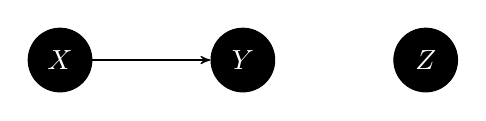
\begin{tikzpicture}
			\node[obs] (X) {$X$} ;
			\node[obs, right=of X] (Y) {$Y$} edge[<-] (X) ;
			\node[obs, right =of Y] (Z) {$Z$} ;
			
		\end{tikzpicture}
		\caption{A false test $Y\not\ind Z$ may lead to the conclusion that the true graph is $X\to Y\to Z$. If this was the only error, the test $Y\ind Z\mid X$ would correct that. But $Y\not\ind Z\mid X$ follows via Graphoid axioms from the marginal tests.}
		\label{fig:graphoid_hurts_correction_example}
	\end{figure}
\end{example}
\paragraph{Error Correction in Spanning Trees}

The following result shows that we can correct errors if we consider more tests than necessary.
To circumvent the issues raise in \cref{ex:graphoid_hurts_correction}, we restrict ourselves to the tests with conditioning set of size one.
This way, we get a set of tests that are not restricted by Graphoid axioms (up to axiom 1) but suffice to identify a spanning tree.
\begin{lemma}
\label{lem:tree_tests_non_graphoid}
		Let $L = \{\CI(X, Y\,|\, Z) :\:X, Y, Z\in V,\, X\neq Y,\, X\neq Z,\, Y\neq Z\}$ such that $\CI(X, Y\mid Z) = \CI(Y, X\mid Z)$ for all distinct $X, Y, Z\in V$. 
        Then $L$ contains no contradictions w.r.t. to the Graphoid axioms and $C(L) = L$.
\end{lemma}
Then we can indeed simply pick the \enquote{message} whose encoding has the smallest distance to the received code word, i.e. the tree whose independence model differs the least from the observed one.
%TODO define Markov distance
\begin{proposition}[Error Correction in Trees]
	\label{prop:error_correction_trees}
    Let the set $S = \{(X, Y, Z) :\: X, Y, Z\in V,\, X\neq Y,\, X\neq Z, Y\neq Z\}$.
	Further, let $\cT_n$ be the set of spanning trees with $n\in \N_{> 3}$ nodes, $T^*\in \cT_n$ and $M$ be an independence model with $\MD_S(T^*, M) \le \lfloor \frac{n-1}{2} \rfloor$. Then
	\begin{displaymath}
		T^* = \arg\min_{T\in \cT_n} \MD_S(T, M),
	\end{displaymath}
	i.e. by minimising the Markov-distance to $M$ we can correct  at least $\lfloor \frac{n-1}{2} \rfloor$ errors for any spanning tree $T^*$.
\end{proposition}
\dominik{since you have a result on graph redudancies in trees, you may want to count only those?}


\paragraph{Error Correction in DAGs}
\label{subsec:dags}
The strong graphical assumptions in the previous section enabled us to derive the error correction guarantee in \cref{prop:error_correction_trees}.
It would be desirable to have a similar result for DAGs.
As the following example shows, this is not possible without further restrictions.
\begin{example}
	\label{ex:complete_dag_single_error}
	Let $G$ be a complete DAG over $\bV$, i.e. for $n\in\N_{>1}$ the graph with nodes $\{X_1, \dots, X_n\}= \bV$ and edges $X_i\to X_j$ whenever $i < j$.
	Suppose our tests unfaithfully show $X_{n-1}\ind X_n\mid \bV\setminus\{X_{n-1}, X_n\}$.
	Clearly, this observed independence model would be explained by the graph $G-(X_{n-1}\to X_n)$. % i.e. the complete graph without the edge between $X_{n-1}\to X_n$.
	Even though this is only a single error, there is another graph that perfectly explains the independence model, so without further knowledge we would prefer this graph over $G$.
\end{example}
\looseness=-1One might consider a subset of tests that is known to contain no implications about each other, like we already did in \cref{prop:error_correction_trees}.
As we have seen in \cref{ex:cpc_not_graphoid_redundant}, a potential candidate could be the tests that the CPC algorithm by \citet{ramsey2006adjacency} utilises to orient colliders.
Indeed, \citet{colombo2014order} have proposed to do a majority voting over these tests (although they did not investigate the Graphoid redundancy of these tests).
Clearly, this method is capable of correcting errors.
It would be interesting to characterize further such \enquote{local} criteria, where a subgraph of the learned DAG can be corrected.
But note how \citet{colombo2014order} rely on the assumption that the learned skeleton is correct.
Without such an assumption it is not obvious how a local error correction could be established.
\todo{Better than last version or too defensive?}
%Although this might be a pragmatic assumption in practice, it is not clear why the tests contributing to the skeleton should a priori be more reliable than the ones used to orient edges.

%\dominik{Note that orientation combines independence with dependences, which is a weird thing that maybe no-where else occurs in statistics. There is not type 1 or type 2 error guarantee!}

\looseness=-1A different approach would be to study under which conditions the optimization over \emph{all} tests works.
Indeed, recently there has been a lot of interest in methods like the \emph{sparsest permutation} (SP) algorithm \citep{raskutti2018learning,lam2022greedy,andrews2023fast}, which outputs the sparsest graph among the graphs that can be constructed like in \cref{prop:protocol_graph_markovian} for all permutations of the nodes.
\citet{raskutti2018learning} show that the required assumption is strictly weaker than faithfulness.
Moreover, they postulate a \enquote{statistical/computational trade-off}, i.e. that additional computations can help to reduce statistical uncertainty.
Although they do not formally analyze this statement, the idea is in line with our work.
To emphasise this, we will quickly study SP from the perspective of redundancy.
Note, that SP relies on two aspects: it outputs a DAG $G^*$ if
\begin{enumerate} \todo{replace tests with CI-statements}
\item   there is a topological ordering $\pi^*$ w.r.t. $G^*$ s.t. all tests in $L_{\pi^*}$ are as in $M_{G^*}$.
\item  for all other permutations $\pi'$ there are no less than $|G^*|$ dependences in $L_{\pi'}$.
\end{enumerate}
\looseness=-1Evidently, if (1) fails the algorithm cannot recover from this error.
But in principle, SP can correct arbitrary errors in $L_{\pi'}$, as long as property (2) holds.
If we assume that the underlying independence model is Graphoid, the errors that can occur are already restricted.
\Cref{prop:protocol_graph_markovian} implies that given (1) all \emph{in}dependences are Graphoid redundant and thus we are unlikely to find a contradiction here.
Further, \cref{prop:coupling} also characterizes dependencies that follow from (1).
This means, the errors that the SP algorithm can correct are for example of the kind of \cref{prop:sufficient_cond_non_graphoid}.

\looseness=-1In principle, it would be desirable to have an algorithm that can also handle violations of (1).
In the following we will propose an assumption and an algorithm that achieves this in some cases, but at the price of being even more expensive than the SP algorithm.
The main purpose of this is not to propose a practical alternative to SP, but rather to demonstrate that the utility of redundant CI-statements is not tied to a specific algorithm or assumption.
\begin{assumption}[Minimum Markov Distance]
\label{ass:mmd}
	Let $\cG$ be a set of graphical models, $G^*\in\cG$ and $M$ an independence model. 
	We say $G^*$ and $M$ fulfill the \emph{minimum Markov distance assumption} (MMD) iff
	%\begin{displaymath}
		$G^* \in \arg\min_{G\in\cG} \MD(G, M)$.
	%\end{displaymath}
\end{assumption}
%Not surprising, assumption \ref{ass:mmd} is weaker than  faithfulness.
Not surprising, assumption \ref{ass:mmd} is weaker than  faithfulness as \cref{prop:faithfulness_implies_mmd} shows.
Perhaps more interesting, \cref{ex:mmd_holds_sp_not} shows a case where SP fails but MMD still recovers the correct graph.
Yet, MMD is not strictly weaker than the SP algorithm, as \cref{ex:sp_works_mmd_not} demonstrates.
\todo{Split senctences and put between examples?}
\begin{proposition}
\label{prop:faithfulness_implies_mmd}
\todo{Introduce $\cG$ again?}
	Let $G^*\in\cG$ be a graphical model and $M$ be an independence model that is Markovian and faithful to $G^*$.
	Then $G^*$ and $M$ also fulfill MMD.
	Further, there are independence models $M$ that fulfill MMD 
    relative to $G$
    but are not Markovian and faithful to any graph $G\in \cG$.
\end{proposition}
%Perhaps more interesting, there are cases where SP fails but MMD still recovers the correct graph.
\begin{example}[MMD holds but not SP]
\label{ex:mmd_holds_sp_not}
    Consider an independence model $M$ that is Markovian and faithful to the graph $G$ in \cref{fig:sp_fails_against_mmd} except for the independences $X_1\ind X_2\mid X_4$ and $X_2\ind X_3\mid X_1$.
    It can be verified easily that $G$ and $M$ fulfill MMD with $
    \MD(G, M) = 1$.
    But SP cannot recover $G$, as the algorithm would output $G - (X_2\to X_3)$.
	\label{ex:sp_fails_against_mmd}
				\begin{figure}[htp]
		\centering
		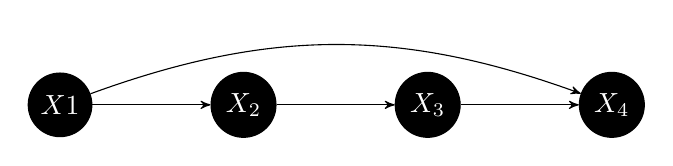
\begin{tikzpicture}
			\node[obs] (X1) {$X1$} ;
			\node[obs, right=of X1] (X2) {$X_2$} edge[<-] (X1) ;
			\node[obs, right=of X2] (X3) {$X_3$} edge[<-] (X2) ;
            \node[obs, right=of X3] (X4) {$X_4$} edge[<-] (X3) ;
			\draw (X1) edge[->, bend left=20] (X4);
		\end{tikzpicture}
		\caption{If this graph is the ground truth but we have the unfaithful independences $X_1\ind X_2\mid X_4$ and $X_2\ind X_3\mid X_1$, MMD is fulfilled but SP outputs a different graph.}
		\label{fig:sp_fails_against_mmd}
	\end{figure}
\end{example}
%Yet, MMD is not strictly weaker than the SP algorithm.
\begin{example}[SP works but not MMD]
\label{ex:sp_works_mmd_not}
	Consider the graph $G$ with nodes $X, Y, Z$ but no edges.
    Assume further that due to false positive CI-tests we get the independence model %\footnote{Note, that $M$ is not Graphoid.} 
    $M$ with $Y\not\ind Z,\, X\not\ind Y\ |\  Z$,\, $X\not\ind Z\ |\  Y$ 
    and independence otherwise (Note, that this model is not Graphoid).
    Clearly $\MD(G, M) = 3$. But for the graph $G'$ with the additional edge $Y\to Z$ we have $\MD(G', M) = 2$, so $G$ and $M$ do not fulfill MMD.
    Yet,  SP would return $G$.
\end{example}

%\begin{itemize}
%	\item MPC \cite{colombo2014order} does majority voting over purely graphical CIs
%	\item Eulig et al propose as baseline to compare against similar graphical models (not clear, improve argument)
%	\item SP algo checks graphically redundant tests
%\end{itemize}

\begin{figure*}[t]
    \centering
    \subfloat[The $p$-values of different CI-tests that are implied by known tests to be either dependent or independent.]{
	\includegraphics[width=.3\linewidth]{img/p_values_graphoid_tests_new.png}
	%\caption{}
	\label{fig:p_values_redundant}
    }\hspace{1em}
    \subfloat[Incorrect predictions of purely graphically redundant CI-statements for different models and data.]{
    \includegraphics[width=.27\linewidth]{img/graphically_red_test_two_datasets_new.png}
	%\caption{}
	\label{fig:graphically_redundant_two_datasets}
    
    }\hspace{1em}
    \subfloat[Structural Hamming distance for simplified PC algorithm and MMD algorithm from \cref{prop:error_correction_trees}. MMD outperforms PC.]{
    \includegraphics[width=.3\linewidth]{img/mmd_vs_pc_new.png}
	%\caption{}
	\label{fig:tree_discovery}
    }
    \caption{Experimental results\vspace{-\baselineskip}}
    \label{fig:enter-label}
\end{figure*}

\section{Experiments}
\looseness=-1In the first experiment, we generated synthetic data from a multivariate Gaussian distribution with four variables 
and conducted several CI-tests (see \cref{sec:experiment_details} for more details on all experiments).
Before each test, we check with the \texttt{Z3} solver \citep{z3} whether the result is already implied by the previous tests via Graphoid axioms.
If so, we track what result the axioms imply and the resulting $p$-value of a CI-test.
As we can see in \cref{fig:p_values_redundant}, the $p$-values mostly follow the predictions.
This corroborates our hypothesis that Graphoid redundant tests provide little additional information and could thus give a false impression of evidence. 


\looseness=-1In the next experiment, %we wanted to see how well the purely graphically redundant tests can indicate if a model does not fit the data.
%To this end 
we synthetically generated two datasets with four binary variables.
One follows the DAG with edges $X\leftarrow W\to Y$ and $X\to Z\leftarrow Y$ while the other one follows the undirected model with the same skeleton.
%For each dataset we drew parameters uniformly at random, created 5000 samples and repeated the whole experiment 1000 times.
We then learn a DAG and an undirected model with the procedures described in \cref{prop:protocol_graph_markovian,prop:markov_network_markovian} and identify purely graphically redundant CI-statements using \cref{prop:sufficient_cond_non_graphoid}.
We then check whether they hold empirically in the data.
\Cref{fig:graphically_redundant_two_datasets} shows the fraction of these test where the graphical implication and the empirical tests disagree.
We can see that the models  tend to make fewer wrong predictions when they match the respective data generating process (green) than the other model (blue).

\looseness=-1Finally, %we wanted to test, whether the error correction presented in \cref{prop:error_correction_trees} can actually improve the result of graph discovery.
%To this end we 
we generated a multivariate Gaussian distribution that is Markovian to a spanning tree over five nodes. 
We then used the algorithm from \cref{prop:error_correction_trees} (MMD algorithm) and a simplified version of PC to recover the tree. 
As we can see in \cref{fig:tree_discovery}, MMD can indeed profit from considering additional purely graphically redundant tests.

\section{Related Work}
\looseness=-1To the best of our knowledge we are the first to study how the graphical constraints on CI-statements can be used to \emph{detect} and \emph{correct} errors in graph discovery, although e.g.  \citet{ramsey2006adjacency,colombo2014order} have noted that some special CI-statements can achieve this.
The restrictiveness of graphical causal models w.r.t. to their entailed independence models has been noted by \citet{tsamardinos2012towards,janzing2023reinterpreting} and in terms of structural causal models by \citet{gresele2022causal}.
Building on these insights \citet{faller2024self,schkoda2024cross} have also proposed to falsify causal models by exploiting these constraints.
%Particularly, they leverage that graphical models on subsets of the variables can entail constraints for the conditional independences in the joint distribution of all variables.
They highlight the distinction between constraints from the graphical model and from probability theory (via the probabilistic marginal problem),
yet we are the first to highlight the importance of this distinction for CI-tests on a single observed dataset.
\citet{bromberg2009improving} have also noted that contradictions between CI-tests can be corrected to improve discovery results, yet they focus on violations of the Graphoid axioms, which we have argued to be of lesser interest.
%Further, \citet{faller2024self} argue that causal discovery algorithms should strive to be stable w.r.t. to the addition of variables.
\citet{russo2024argumentative} propose to use symbolic reasoning to resolve conflicts in the provided CI-statements but do not make the distinction between graphically and probabilistically redundant tests.\todo{Need to understand this one better.}


%There are classical results in numerics on the condition of matrices \cite{???}.
%But our problem is different as it has a more discrete character.
%In discrete optimization there is a wide literature on \emph{stability} of optimization problem \cite{sotskov1995some}. \textcolor{red}{Need more}.
%But they are more interested in algorithmic aspects (calculating other solutions from an existing one), where we are striving to correct errors.

\looseness=-1There is also a vast literature on making discovery of graphical models robust against statistical uncertainty.
E.g. \citet{kalisch2007estimating} propose a stronger version of faithfulness under which the PC algorithm is uniformly consistent, while \citet{bhattacharyya2021near} show finite-sample bounds for tree learning.
\citet{strobl2016estimating,li2009controlling} use techniques from multi-hypothesis testing to control the error rate of edges. %(see also papers of Tsamardinos in there).
%\todo{Add following and previous line back in}
\citet{kalisch2008robustification, harris2013pc} study how to make PC more robust towards violations of parametric assumptions, while \citet{kim2024causal} use Graphoid axioms to conduct a set of tests that is equivalent it terms of their graphical implications but statistically better conditioned.
%\cite{cano2008score,abellan2006some} propose miscellaneous modifications of the PC algorithm. 
%Also cite this technical report that proposes to use sep set with maximal $p$ value and conservative PC.

\looseness=-1\citet{zhang2016three} argue that the faithfulness assumption serves three functions in graph discovery.
%It makes the problem uniquely solvable in many cases, it reduces the complexity of the problem algorithmically and it makes the problem statistically more tractable.
Our work can be interpreted as adding a fourth \enquote{face} to their three faces of faithfulness by showing that in many cases we get error detection and correction properties only through graphical assumptions that are stronger than the laws of probability, such as faithfulness.
%\dominik{explain in what sense}

\section{Discussion}
\looseness=-1We have demonstrated that additional conditional independence tests can be used to falsify graphical models and to improve discovery results.
We have defined different notions of redundancy to distinguish between CI-statements that are already implied by the laws of probability and the ones that follow only from graphical assumptions.
As the latter ones are more useful for the detection and correction of errors in graph discovery, we have characterised conditions where we have this purely graphical redundancy and conditions under which we only have Graphoid redundancy.

\looseness=-1
Our work shows that numerous correctly predicted CI-statements only provide evidence if they represent independent degrees of freedom of the underlying distribution.
This means that the mere number of correct CI-statements paints a superficial image and cannot corroborate a model.
%This work is supposed to foster a better understanding of how graphical models should be evaluated and that it is not trivial to decide what constitutes evidence for or against a model.
%This understanding is imperative to develop further  methods for falsification and make algorithms more robust.
%Moreover, 
We think that these insights can be a first step towards methods that not only correct errors but also allow to define confidence regions outside of which a model should be rejected, as the model differs to much from the observed evidence.
%\todo{Say more that this paper shows how difficult it is to define proper distance between graphs and independence models. But if we had one we can could also not just correct errors but also define acceptable regions}

\todo{8 Pages limit}

\begin{acknowledgements} % will be removed in pdf for initial submission,
						 % (without ‘accepted’ option in \documentclass)
                         % so you can already fill it to test with the
                         % ‘accepted’ class option
We thank Elke Kirschbaum and William Roy Orchard for helpful discussions and proofreading.
Philipp M. Faller was supported by a doctoral scholarship of the Studienstiftung des deutschen Volkes (German Academic Scholarship Foundation).
This work does not relate to Dominik Janzing's position at Amazon.
\end{acknowledgements}


\bibliography{paper}

\newpage

\onecolumn

\title{On Different Notions of Redundancy in Conditional-Independence-Based Discovery of Graphical Models\\(Supplementary Material)}
\maketitle

\appendix
\section{Detailed Definitions}
\label{sec:further_definitions}
We denote a random variable with upper case letter $X$. 
A set of random variables is denoted with bold face letters $\bX$.
For single variables and sets of variables we write the attained values with lower case letter $x$ and the domain with calligraphic letter $\cX$,

A \emph{graph} $G$ is a tuple $(\bV, \bE)$, where $\bV$ is a finite set of nodes and $\bE \subseteq \bV\times \bV$ is the set of edges.
We say $G$ is \emph{undirected} if $\bE$ is a symmetric relation.
To emphasise the direction of an edge we also write $X\to Y$ for $(X, Y)\in \bE$, $X\leftarrow Y$ when $(Y, X)\in \bE$ and $X-Y$ when the graph is undirected and $(X, Y)\in \bE$.
We slightly abuse notation and write $(X\to Y)\in G$ if $(X, Y)\in \bE$ and analogously for $X\leftarrow Y$ and $X-Y$.
We denote the graph $G - (X\to Y) := (\bV, \bE\setminus\{(X, Y)\})$.
We say two nodes $X, Y\in \bV$ are \emph{adjacent} if we have $(X, Y)\in \bE$ or $(Y, X)\in \bE$ and we denote with $\Adj(X)$ the set of nodes that are adjacent to $X$.
$\PA(Y)$ denotes the set of nodes $X\in \bV$ such that $(X, Y)\in \bE$. 
A \emph{path} $p=(X_1, \dots, X_n)$ is a sequence of $n\in \N_{>1}$ nodes such that $X_i\in \bV$ for $i=1, \dots, n$ and $X_i\in \Adj(X_{i+1})$ for $i=1, \dots, n-1$.
Further, $p$ is called a \emph{cycle} if $X_1=X_n$.
If a graph contains no cycles it is called a \emph{directed acyclic graph} (DAG).
If in an undirected graph $G$ any distinct nodes $X, Y\in \bV$ are connected by at most one node-disjoint path, $G$ is called a \emph{tree}.
If it is exactly one path, $G$ is called a \emph{spanning tree}.
For a DAG $G=(\bV, \bE)$ we define the \emph{skeleton} of $G$ as the undirected graph $H=(\bV, \bE')$, with $(X, Y)\in \bE'$ if $(X, Y)\in \bE$ or $(Y, X)\in \bE$, for $X, Y\in \bV$.
For all graphs $G=(\bV, \bE)$ we denote $|G| := |\bE|$.

Let $\bV$ be a set of random variables.
We call a set $M\subset \cP(\bV)$ an \emph{independence model}\footnote{Note, that \citet{bouckaert1995bayesian} formally distinguish between an \emph{independence} and \emph{dependence} model. For our discussion it should suffice to  consider the latter only implicitly.} if all $(\bX, \bY, \bZ) \in M$ are disjoint and $\bX$ and $\bY$ are not empty.
Then we say $\bX$ is \emph{independent} from $\bY$ given $\bZ$ and write $\bX\ind_{\mspace{-8mu}M}\bY\mid \bZ$, where we often omit the subscript.
If $(\bX, \bY\, \bZ)$ is not in $M$ we say $\bX$ is \emph{dependent} on $\bY$ given $\bZ$ and write $\bX\not\ind \bY\mid \bZ$.
A \emph{CI-statement} is a quadruple of $\bX, \bY, \bZ$ and a boolean value, indicating whether the independence holds.
For a set of CI-statements $L$ we slightly abuse notation and write $L\subseteq M$ if for $(\bX, \bY, \bZ, b)\in L$ we have $b=((\bX,\bY,\bZ)\in M$).
We also sometimes write a CI-statement as function $\CI: \bX, \bY, \bZ\mapsto b$ or $\bX \ind \bY\mid \bZ$ if $(\bX, \bY, \bZ)\in M$ and $\bX \not\ind \bY\mid \bZ$ if $(\bX, \bY, \bZ)\not\in M$.
As we note before, with \emph{in}dependences we refer to statements of the form $\bX\ind \bY\mid \bZ$ and with dependences to $\bX\not\ind \bY\mid \bZ$, while with CI-statement we refer to both of them.

A probability distribution over $\bV$ entails an independence model by the standard definition of probabilistic conditional independence, i.e. $\bX\ind \bY\mid \bZ$ w.r.t. the distribution $P$ iff 
\begin{displaymath}
    P(\bX = \bx, \bY=\by\mid \bZ=\bz) = P(\bX=\bx\mid \bZ=\bz)\cdot P(\bY=\by\mid \bZ=\bz),
\end{displaymath}
for all $\bx\in\cX, \by\in \cY, \bz\in\mathcal{Z}$.
We often refer to the distribution and its independence model interchangably.

We can also use graphs to represent independence models.
First we define a graphical notion that will then correspond to conditional independence.
Let $G$ be an undirected graph with nodes $\bV$ and $\bX, \bY\, \bZ\subseteq \bV$ be disjoint with $\bX\neq \emptyset \neq \bY$.
We say $\bX$ and $\bY$ are \emph{separated} given $\bZ$ if every path from $X\in \bX$ to $Y\in \bY$ contains a node in $\bZ$.
If a path contains no node in $\bZ$ we say it is \emph{active}.
For a DAG $G=(\bV, \bE)$, and a path $p=(X_1, \dots, X_n)$ in $G$ we say $X_i$ is a \emph{collider} on $p$ if $(X_{i-1}\to X_i), (X_i \leftarrow X_{i+1}) \in \bE$, for $n\in \N_{>2}, X_1, \dots, X_n \in \bV, i\in \{2, \dots, n-1\}$.
We say a path $p$ is \emph{active} given $\bZ$ if for all colliders $C$ on $p$ a descendant of $C$ or $C$ itself is in $\bZ$.
The set $\bX$ and $\bY$ are \emph{$d$-separated} if there are no $X\in \bX$ and $Y\in \bY$ such that there is an active path given $\bZ$ between $X$ and $Y$.
Now we denote a model induced by a graph $G$ as $M_G$.
For an undirected graph $G$ we define $(\bX, \bY, \bZ) \in M_G$ iff $\bX$ is separated from $\bY$ given $\bZ$.
For DAGs $(\bX, \bY, \bZ) \in M_G$ iff $\bX$ is $d$-separated from $\bY$ given $\bZ$.
By \emph{graphical model} we refer to \emph{either} an undirected graph or a DAG (and its respective independence model).
As we have noted before, we restrict our attention to undirected graphs and DAGs.
But our insights can be applied to any model that is equipped with a notion of independence between nodes, such as chain graphs \citep{lauritzen1996graphical}, completed partial DAGs, maximal ancestral graphs, partial ancestral graphs \citep{spirtes2000causation} or acyclic directed mixed graphs \citep{richardson2003markov}.
If for two graphs $G, G'$ we have $M_G = M_{G'}$ we say $G$ and $G'$ are \emph{Markov-equivalent} and for any DAG $G$ we call the set of DAGs that are Markov equivalent to $G$ the \emph{Markov-equivalence class} of $G$.

A graph is \emph{Markovian} to an independence model $M$ if $(\bX, \bY, \bZ) \in M_G \implies(\bX, \bY, \bZ) \in M$ and it is \emph{faithful} if $(\bX, \bY, \bZ) \in M \implies (\bX, \bY, \bZ) \in M_G$.
Again, we slightly abuse notation and say $G$ is Markovian to a set of CI-statements $L$ when all \emph{in}dependences in $G$ are contained in $L$.
%As a convenient shorthand we also use 
%\begin{displaymath}
% $   \CI(\bV) := \{(X, Y, \bZ) : X, Y\in \bV, \bZ\subseteq \bV\setminus\{X, Y\}, X\neq Y\}$.
%\end{displaymath}
For independence models $M, M'$ over $\bV$ we define the \emph{Markov distance} w.r.t. $S\subseteq \CI(V)$ via
%\begin{displaymath}
 $   \MD_S(M, M') = \sum_{s\in S} \mathbb{I}\left[(s\in M) \neq (s\in M')\right]$.
%\end{displaymath}
We omit the subscript if $L=\CI(\bV)$.
%In this case, \citet{wahl2024metrics} call this \emph{s/c-metric} and show that it is a proper metric.
We extend the definition to a graph $G$ by considering the induced independence model $M_G$, i.e. we define $\MD_S(G, M) = \MD_S(M_G, M)$ and $\MD_S(M, G) = \MD_S(M, M_G)$.

\section{Proofs}
\label{sec:proofs}
\begin{proof}[Proof for \cref{prop:continuity_partial_corr}]
    In this proof we will mainly use the recursive characterisation of partial correlations, i.e. for real values random variables $X, Y$ and set of real-valued random variables $\bZ$ with $Z'\in \bZ$ we have
    \begin{displaymath}
        \rho_{X,Y\cdot \bZ} = \frac{\rho_{X, Y\cdot \bZ\setminus \{Z'\}} - \rho_{X, Z'\cdot \bZ\setminus\{Z'\}}\rho_{Z', Y\cdot \bZ \setminus \{Z'\}}  }{\sqrt{1- \rho_{X, Z' \cdot \bZ\setminus\{Z'\}}^2}\sqrt{1- \rho^2_{Z',Y \cdot \bZ\setminus\{Z'\}}}},
    \end{displaymath}
    where this should be read as  
    \begin{displaymath}
        \rho_{X,Y\cdot \bZ} = \frac{\rho_{X, Z} - \rho_{X, Z'}\rho_{Z', Y}}{\sqrt{1- \rho_{X, Z'}^2}\sqrt{1- \rho^2_{Z',Y}}},
    \end{displaymath}
    when $\bZ$ only contains $Z'$.
    To get the correspondence to the Graphoid axioms we define the absolute partial correlation between non-empty sets of variables $\bX, \bY$ given $\bZ$ as 
    \begin{displaymath}
        |\rho_{\bX,\bY\cdot \bZ}| := \max_{X\in \bX, Y\in \bY} |\rho_{X,Y\cdot \bZ}| 
    \end{displaymath}

    Now let $X, Y, Z, W$ be real-valued random variables.
    From the definitions it is clear that 1) and 2) hold trivially.
    For 3) let $\epsilon > 0$ and $|\rho_{X,Y\cup W\cdot \bZ}| <\epsilon$, i.e. we have $|\rho_{X,Y\cdot \bZ}| < \epsilon$ and $|\rho_{X,W\cdot \bZ}| < \epsilon$ by definition.
    Since partial correlations are bounded by one, there is a $\delta > 0$ with $\rho_{Y, W\cdot Z} \le \delta$. Then we get
    \begin{displaymath}
        |\rho_{X,Y\cdot Z\cup W} |  = \left|\frac{\rho_{X, Y\cdot Z} - \rho_{X, W \cdot Z}\rho_{Y, W\cdot Z}}{\sqrt{1- \rho_{X, W \cdot Z}^2}\sqrt{1- \rho^2_{Y, W\cdot Z}}}\right|
        \le \frac{\epsilon(1 - \delta)}{\sqrt{1- \epsilon^2}\sqrt{1- \delta^2}}.
    \end{displaymath}
    Since $\epsilon, \delta\in (0, 1]$, we have $1-\epsilon^2 \ge (1-\epsilon)^2$ and thus
    \begin{displaymath}
        |\rho_{X,Y\cdot Z\cup W} |  \le\frac{\epsilon(1 - \delta)}{\sqrt{(1- \epsilon)^2}\sqrt{(1- \delta)^2}}
        = \frac{\epsilon(1 - \delta)}{(1- \epsilon)(1- \delta)}
        = \frac{\epsilon}{1-\epsilon} \le 2\epsilon,
    \end{displaymath}
    where the last inequality holds due to $\epsilon \le 1/2$.
    The argument for $|\rho_{X,W\cdot Z\cup Y} |$ works symmetrically.

    For 4) assume $|\rho_{X,Y\cdot Z}| \le \epsilon$ and $|\rho_{X,W\cdot Z\cup Y}| \le \epsilon$.
    By our definition it remains to show $\rho_{X,W\cdot Z\cup Y}\le 2\epsilon$.
    From the second antecedent we get
    \begin{displaymath}
        \epsilon \ge |\underbrace{\rho_{X,W\cdot Z} - \rho_{X,Y\cdot Z}\rho_{W,Y\cdot Z}}_{:=a}|.
    \end{displaymath}
    If $a>0$ we have 
    \begin{displaymath}
        \rho_{X,W\cdot Z\cup Y} \le \epsilon + \rho_{X,Y\cdot Z}\rho_{W,Y\cdot Z} \le \epsilon + \epsilon \cdot |\rho_{W,Y\cdot Z}| \le \epsilon + \epsilon = 2\epsilon.
    \end{displaymath}
    Similarly for $a< 0$ we get
    \begin{displaymath}
        \rho_{X,W\cdot Z\cup Y} \le \epsilon - \rho_{X,Y\cdot Z}\rho_{W,Y\cdot Z} \le \epsilon + \epsilon \cdot |\rho_{W,Y\cdot Z}| \le 2\epsilon.
    \end{displaymath}

    For 5) we additionally assume that $|\rho_{W,Y\cdot Z}| \le 1 -\epsilon$. Now let $|\rho_{X,Y\cdot Z\cup W}| \le \epsilon$ and $|\rho_{X,W\cdot Z\cup Y}| \le \epsilon$. Then we have
    \begin{displaymath}
       \epsilon \ge |\rho_{X,Y\cdot Z\cup W} |  = \frac{|\rho_{X,Y\cdot Z} - \rho_{X,W\cdot Z}\rho_{Y,W\cdot Z}|}{\sqrt{1- \rho_{X,W\cdot Z}^2}\sqrt{1- \rho_{Y,W\cdot Z}^2}} \ge |\underbrace{\rho_{X,Y\cdot Z} - \rho_{X,W\cdot Z}\rho_{Y,W\cdot Z}}_{:= a}|
    \end{displaymath}
    and similarly
    \begin{displaymath}
       \epsilon \ge |\rho_{X,W\cdot Z\cup Y} |  = \frac{|\rho_{X,W\cdot Z} - \rho_{X,Y\cdot Z}\rho_{W,Y\cdot Z}|}{\sqrt{1- \rho_{X,Y\cdot Z}^2}\sqrt{1- \rho_{W,Y\cdot Z}^2}} \ge |\underbrace{\rho_{X,W\cdot Z} - \rho_{X,Y\cdot Z}\rho_{W,Y\cdot Z}}_{:= b}|.
    \end{displaymath}
    Now suppose $a, b  \ge 0$. Then we get
    \begin{displaymath}
        \epsilon + \rho_{X,W\cdot Z}\rho_{Y,W\cdot Z} \ge \rho_{X,Y\cdot Z} \quad \text{ and } \quad \epsilon + \rho_{X,Y\cdot Z}\rho_{W,Y\cdot Z} = \rho_{X,W\cdot Z}.
    \end{displaymath}
    From inserting the second inequality into the former we get
    \begin{align*}
        \rho_{X,Y\cdot Z} &\le \epsilon + (\epsilon + \rho_{X,Y\cdot Z}\rho_{W,Y\cdot Z}) \rho_{Y,W\cdot Z} = \epsilon + \epsilon\rho_{Y,W\cdot Z} + \rho_{X,Y\cdot Z}\rho_{Y,W\cdot Z}^2 \\
        \rho_{X,Y\cdot Z} (1 - \rho^2_{W,Y\cdot Z}) &\le \epsilon + \epsilon \rho_{W,Y\cdot Z}\\
        \rho_{X,Y\cdot Z} & \le \frac{\epsilon}{(1 - \rho^2_{W,Y\cdot Z})} + \frac{\epsilon \rho_{W,Y\cdot Z}}{(1 - \rho^2_{W,Y\cdot Z})} \le \frac{\epsilon}{(1 - \rho^2_{W,Y\cdot Z})} + \frac{\epsilon^2}{(1 - \rho^2_{W,Y\cdot Z})}.
    \end{align*}
    Since we have assumed $|\rho_{W,Y\cdot Z}| \le 1 -\epsilon$ we also have $1 - \rho^2_{W,Y\cdot Z} \ge 1 - \epsilon$ and thus
    \begin{displaymath}
        \rho_{X,Y\cdot Z} \le \frac{\epsilon}{1-\epsilon} + \frac{\epsilon^2}{1-\epsilon} \le 4\epsilon.
    \end{displaymath}
    The other combinations of sings of $a$ and $b$ work analogously, just as the case for $\rho_{X,W\cdot Z}$.
\end{proof}

\begin{proof}[Proof for \cref{prop:sufficient_cond_non_graphoid}]
\todo{Add visualization}
Let $L$ be a set of CI-statements over variables $\bV$ and $s = (X\not\ind Y \mid \bZ)\not\in L$ for $(X, Y, Z)\in \CI(\bV)$.
	We will prove the statement by constructing a Graphoid independence model that contains all CI-statements in $L$ but not $X\not\ind Y \mid Z$ by building a distribution that is Markovian but not faithful to a DAG.
	
	If $X$ and $Y$ are only $d$-connected given $Z$ by a direct edge, we set $G' = (V, E\setminus\{(X, Y), (Y, X)\})$. 
	
	Otherwise, let $N(X\sim Y\mid \bZ)$ be the set of nodes on the active paths between $X$ and $Y$ given $\bZ$ (without $X$ and $Y$).
	We construct a new graph $G' = (V', E')$ with more nodes and more edges.
	First, add all nodes in $V\setminus N(X\sim Y\mid \bZ)$ to $V'$.
	For each $W\in N(X\sim Y\mid \bZ)$, we add nodes $W_1, W_2$ to $V'$.
	For all edges $W \to W'$ with $W, W' \in N(X\sim Y\mid \bZ)$, add the edges $W_1 \to W_1'$ and $W_2\to W_2'$.
	If $W'\in V\setminus N(X\sim Y\mid \bZ)$ add $W_1\to W'$ and $W_2\to W'$ and analogously add $W\to W'_1$ and $W\to W'_2$ if $W\in V\setminus N(X\sim Y\mid \bZ)$.
	Finally add $X\to W_1$ and $X\leftarrow W_1$ whenever $X\to W$ or $X\leftarrow W$ for $W\in  N(X\sim Y\mid \bZ)$ and $Y\to W_2$ and $Y\leftarrow W_2$ respectively.
	
	Clearly, in this graph we have $X\perp_{G'} Y\mid \bZ'$, where $\bZ'$ contains all nodes in $\bZ\setminus N(X\sim Y\mid \bZ)$ and $W_1, W_2$ for $W\in \bZ\cap N(X\sim Y\mid \bZ)$.
	It is straight forward to construct a distribution that is Markovian and faithful to $G'$ and is non-negative.
	
	Moreover, if we construct a graph $G''$ by considering every pair $W_1, W_2$ for $W\in N(X\sim Y\mid \bZ)$ as a vector-valued variable (and keep the canonical mapping between node names $W=(W_1, W_2)$), this graph again, contains all CI-statements we had in $L$ but $X\perp_{G''} Y\mid \bZ$.
	Thus, also the probability distribution we get from $G'$ by interpreting $(W_1, W_2)$ as vector-valued variables contains these CI-statements.
	Further, it is also non-negative if the distribution w.r.t. $G'$ was and therefore its independence model is Graphoid.
	
	To see this, let $(A\ind B\mid \bC)\in C(L)$.
	Since $G$ was Markovian to $L$, there was no active path in $G$ given $\bC$ connecting $A$ and $B$.
	And because we did not add an edge between nodes that were disconnected and we did not introduce any colliders between these nodes, we also have no active path in $G''$.
	Now suppose $(A\not\ind B\mid \bC)\in C(L)$.
	By assumption, we have $A\not\perp^s_{G} B\mid \bC$, i.e. there is an active path between $A$ and $B$ given $\bC$ that does not contain any subpath from $X$ to $Y$ that is active given $\bZ$.
	As we only modified the paths between $X$ and $Y$ that are active given $\bZ$, the path between $A$ and $B$ is still active.
    So we also still have $A\not\perp_{G''} B\mid \bC$.
	
	It now suffices to note that every non-negative distribution (and therefore especially the one we just constructed) implies a Graphoid independence model. 
\end{proof}

\begin{proof}[Proof for \cref{lem:tree_tests_non_graphoid}]
    Let $L = \{\CI(X, Y\mid Z) : X, Y, Z\in V, X\neq Y, X\neq Z, Y\neq Z\}$ such that $\CI(X, Y\mid Z) = \CI(Y, X\mid Z)$ for all distinct $X, Y, Z\in V$. 
    Then for any CI-statement $\CI(X, Y\mid Z)\in L$, only axiom 1 from \cref{def:graphoid} is applicable, since all the other axioms require at least on of the operands to be a set of size larger than one, which we don't have in $L$.
    By assumption, we have no contradictions between the statements in $L$ and the statements that follow from axiom 1.
    And also $L$ contains all statements that can be derived with axiom 1.
\end{proof}

\begin{proof}[Proof for \cref{prop:error_correction_trees}]
    Let $S = \{(X, Y, Z) : X, Y, Z\in V, X\neq Y, X\neq Z, Y\neq Z\}$.
	Further let $T^*\in \cT_n$ and let $M$ be an independence model with $\MD_S(T^*, M) \le \lfloor \frac{n-1}{2} \rfloor$ for $n\in \N_{> 3}$. 
    To arrive at a contradiction we assume
	\begin{equation}
		\MD_S(T', M) < \MD_S(T^*, M), \label{eq:proof_tree_correction}
	\end{equation}
    for some tree $T'\in\cT_n$ with $T'\neq T^*$.
    Since the graphs differ and both are trees, there are nodes $X, Y$ that were connected by a direct edge in $T^*$ but are not in $T'$.
    But since they are spanning trees there still exists a path of length $k\in \N_{>1}$ between $X$ and $Y$ in $T'$.
    So there is at least one node $Z$ such that we have $X\perp_{T'} Y\mid Z$ but $X\not\perp_{T^*} Y\mid Z$, because of the edge between $X$ and $Y$ in $T^*$.
    So we have at least one CI-statement difference between $T'$ and $T^*$.
    For the second difference, there are two cases how $Z$ is connected to $X$ in $T^*$.
    \begin{enumerate}
        \item If $Y$ lies between $X$ and $Z$, i.e. $X-Y\overset{*}{-}Z$ we get $X\not\perp_{T'}Z\mid Y$ but $X\perp_{T^*}Z\mid Y$.
        \item If $X$ lies between $Y$ and $Z$, i.e. $Z\overset{*}{-}X-Y$ we get $Z\not\perp_{T'} Y
        \mid X$ but $Z\perp_{T^*} Y\mid X$.
    \end{enumerate}
    So in any case we have another difference between $T^*$ and $T'$.

    W.l.o.g. we can assume that $Z$ is the node closest to $X$ on the path between $X$ and $Y$, i.e. the node that has a direct edge to $X$.
    Now let $W$ be another node (which exists, because $n>3$).
    There are three cases how this node can be connected to $X$ along the unique path in $T'$.
    \begin{enumerate}
        \item If $Y$ is between $Z$ and $W$, i.e. if we have 
        \begin{displaymath}
            X - Z \overset{*}{-} Y \overset{*}{-} W.
        \end{displaymath}
        Then we have $X\perp_{T'}W\mid Z$ but $X\not\perp_{T^*} W\mid Z$, since in $T^*$ we had the direct edge from $X$ to $Y$.
        \item If $Y$ does not lie on the paths between $X$ and $W$ and $X$ not on the one between $Y$ and $W$, i.e. if we have the structure in \cref{fig:proof_error_correction_tree}, we will further subdivide this into two subcases depending on $T^*$.
        \begin{enumerate}
            \item In $T^*$ we have $Y$ between $X$ and $W$, i.e. $X-Y\overset{*}{-}W$. Then $X\not\perp_{T'}W\mid Y$ but $X\perp_{T^*}W\mid Y$.
            \item In $T^*$ we have $X$ between $Y$ and $W$, i.e. $W\overset{*}{-}X-Y$. Then we have $Y\not\perp_{T'}W\mid X$ but $Y\perp_{T^*}W\mid X$.
        \end{enumerate}
        \item If $X$ is between $W$ and $Y$, i.e.
        \begin{displaymath}
            W \overset{*}{-} X - Z \overset{*}{-} Y.
        \end{displaymath}
        Then this case works symmetrically to the first one.
    \end{enumerate}
    Since we chose $W$ arbitrarily, we can repeat this for every node other than $X, Y, Z$.
    This means, we get $n-3$ more contradictions between the independence model of $T^*$ and $T'$.
    So overall we have $n-1$ CI-statements where $T'$ and $T^*$ disagree.
    So even if $T'$ fits all the $\lfloor \frac{n-1}{2} \rfloor$ tests where $T^*$ and $M$ differ, it will also differ by another $\lceil \frac{n-1}{2} \rceil$ statements from $T^*$ and therefore also from $M$.
    This is a contradiction to \cref{eq:proof_tree_correction}.
    
    \begin{figure}[htp]
		\centering
		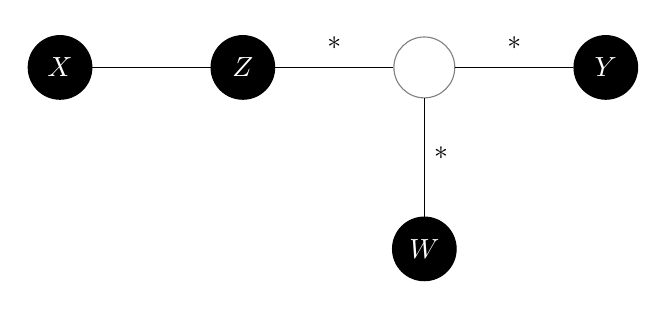
\begin{tikzpicture}
			\node[obs] (X) {$X$} ;
			\node[obs, right=of X] (Z) {$Z$} edge[-] node[above]{} (X) ;
            \node[vardashed, right =of Z] (empty) {} edge[-] node[above]{*} (Z);
			\node[obs, right =of empty] (Y) {$Y$} edge[-] node[above]{*} (empty);
            \node[obs, below =of empty] (W) {$W$} edge[-] node[right]{*} (empty);
			
		\end{tikzpicture}
		\caption{Visualization how the node $W$ from the proof of \cref{prop:error_correction_trees} can be connected to $X$ and $Y$ in case 2 of the proof.}
		\label{fig:proof_error_correction_tree}
	\end{figure}
\end{proof}

\begin{proof}[Proof of \cref{prop:faithfulness_implies_mmd}]
    Let $G^*\in\cG$ be a graphical model and $M$ be an independence model that is Markovian and faithful to $G^*$.
    Then by definition we have $M = M_{G^*}$.
    This means $\MD(M, G^*) = 0$ and since the Markov-distance is non-negative, surely $\MD(M, G^*) \le \MD(M, G)$ for any DAG $G$.
    To see that there are cases where MMD holds but $M$ is not faithful to any DAG, consider again \cref{ex:mmd_holds_sp_not}.
    For faithfulness, a graph $G$ would have to contain no edge between $X_1$ and $X_2$. But then the dependence $X_1\not\ind X_2$ would violate the Markov property.
    Therefore, there is no DAG that is Markovian and faithful to the given independence model, yet MMD holds.
\end{proof}

\section{Additional Examples}

\begin{example}[Wrong Collider-Structure]
	\label{ex:wrong_v_structure}
	In this example we assume we want to find a graph using the PC algorithm \cite{pearl2009causality}.
	Consider the family of graphs depicted in \cref{fig:wrong_v_structure_gt}.
	Assume there are nodes $Z$ and $X_i$ for $i=0, \dots, k\in\N_{>1}$.
	Further assume all CI-test results are Markovian and faithful to the graph, except for 
	\begin{displaymath}
		X_0\ind Z.
	\end{displaymath}
	Then the algorithm would wrongly detect a collider structure between $X_0, X_1$ and $Z$, as $X_1$ is not in the separating set of $X_0$ and $Z$.
	Then, by application of Meek rules \citep{meek1995causal}, this orientation propagates along the path.
	As in the true graph there is no collider between $X_2, X_1$ and $X_0$, the triplet will not be oriented as collider and by Meek rule R1 the edge $X_1-X_2$ will become $X_1\to X_2$.
	The same argument holds for all further $X_{i+1}, X_i$ with $i>2$, which will cause the algorithm to orient the whole chain of $X_i$ the wrong way around, as visualized in \cref{fig:wrong_v_structure_res}.
	In other words, a single false CI-statement might cause $k+1$ wrongly directed edges.

    If the purpose of the graphical model is simply a concise representation of the CI-statements in the data, this might be acceptable.
    But if the model is interpreted e.g. as a causal model and it is used in some downstream task, this might be worrisome.
    Although graph discovery is already algorithmically expensive, in such cases a practitioner might be willing to incur an additional computational overhead to make the results more robust.
	\begin{figure}[htp]
		\centering
        \subfloat[Ground truth graph]{
        \label{fig:wrong_v_structure_gt}
		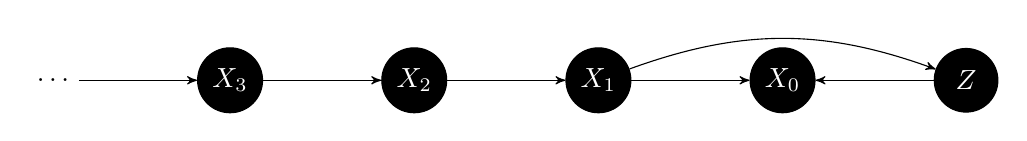
\begin{tikzpicture}
			\node[obs] (X0) {$X_0$} ;
			\node[obs, right=of X0] (Z0) {$Z$} edge[->] (X0) ;
			%\node[obs, above left=of Z0] (Z1) {$Z_1$} edge[->] (Z0) ;
			%\node[obs, above =of Z0] (Z2) {$Z_2$} edge[->] (Z0) ;
			\node[obs, left=of X0] (X1) {$X_1$} edge[->] (X0) ;
			%\draw (X0) edge[->, tabgreen, bend left=10]  (X1);
			%\node[obs,  above right=of X1] (Y0) {$Y_1$} edge[->] (X1) ;
			\node[obs, left =of X1] (X2) {$X_2$} edge[->] (X1) ;
			%\draw (X1) edge[->, tabred, bend left=10]  (X2);
			%\draw (X2) edge[->]  (Y0);
			%\node[obs,  above right=of X2] (Y1) {$Y_2$} edge[->] (X2) ;
			\node[obs, left =of X2] (X3) {$X_3$} edge[->] (X2) ;
			%\draw (X2) edge[->, tabred, bend left=10]  (X3);
			%\draw (X3) edge[->]  (Y1);
			\node[left=of X3] (dots) {$\hdots$} edge[->](X3);
			%\draw (X3) edge[->, tabred, bend left=10]  (dots);
            \draw (X1) edge[->, bend left=20]  (Z0);
		\end{tikzpicture}
        }
        
        \subfloat[Wrongly inferred graph]{
        \label{fig:wrong_v_structure_res}
		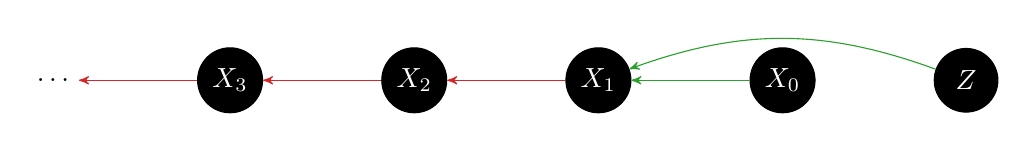
\begin{tikzpicture}
			\node[obs] (X0) {$X_0$} ;
			\node[obs, right=of X0] (Z0) {$Z$};
			%\node[obs, above left=of Z0] (Z1) {$Z_1$} edge[->] (Z0) ;
			%\node[obs, above =of Z0] (Z2) {$Z_2$} edge[->] (Z0) ;
			\node[obs, left=of X0] (X1) {$X_1$} edge[<-, tabgreen] (X0) ;
			%\draw (X0) edge[->, tabgreen, bend left=10]  (X1);
			%\node[obs,  above right=of X1] (Y0) {$Y_1$} edge[->] (X1) ;
			\node[obs, left =of X1] (X2) {$X_2$} edge[<-, tabred] (X1) ;
			%\draw (X1) edge[->, tabred, bend left=10]  (X2);
			%\draw (X2) edge[->]  (Y0);
			%\node[obs,  above right=of X2] (Y1) {$Y_2$} edge[->] (X2) ;
			\node[obs, left =of X2] (X3) {$X_3$} edge[<-, tabred] (X2) ;
			%\draw (X2) edge[->, tabred, bend left=10]  (X3);
			%\draw (X3) edge[->]  (Y1);
			\node[left=of X3] (dots) {$\hdots$} edge[<-, tabred](X3);
			%\draw (X3) edge[->, tabred, bend left=10]  (dots);
            \draw (X1) edge[<-, tabgreen, bend left=20]  (Z0);
		\end{tikzpicture}
        }
		\caption{When the collider-structure $X_0\to X_1\leftarrow Z$ is wrongly identified, all edges $X_{i+1}\to X_i$ will be oriented the wrong way around.}
		\label{fig:graph_v_structure_wrong}
	\end{figure}
	
\end{example}

\begin{example}[PC results can be non-Markovian]
	\label{ex:pc_not_markov}
	Suppose we have an independence model that is Markovian and faithful to the graph in \cref{fig:pc_not_markov_gt}, except for the dependence $X_1\not\ind X_3$ and the independence $X_1\ind X_3\mid Y$.
	Further, suppose we want to recover this graph with the PC algorithm.
	In the first round of the algorithm, it will conduct all marginal independence tests.
    This will give us the intermediate skeleton in \cref{fig:pc_not_markov_intermediate}.
	In the following rounds, the algorithm will conduct all tests with conditioning set of size one and two, which will result in the graph in \cref{fig:pc_not_markov_undirected}.
	But now in the orientation phase, we have conflicting evidence for the existence of colliders and depending on how exactly the algorithm resolves them, we will get different results.
	E.g. in the default implementation in \texttt{causal-learn} \citep{zheng2024causal} the algorithm simply picks the first orientation according to the (non-predetermined) ordering in which it conducts the CI-tests.
	Suppose, the algorithm first checks whether the unshielded triplet $X_1-Y-X_2$ is a collider.
    This is the case, as $Y$ is not in the separation set of $X_1$ and $X_2$, which is the empty set.
    The same holds for $X_2$ and $X_3$.
    If the algorithm sticks with these orientations, it ignores that $Y$ is indeed member of all separating sets of $X_1$ and $X_3$.
    Therefore, it would output the graph in \cref{fig:pc_not_markov_gt}.
    But note, that this graph does imply $X_1\ind X_3$ which does not hold in our independence model.
    It can be checked (e.g. with \texttt{Z3}) that the CI-tests that we used are indeed a valid Graphoid.	
	\begin{figure}[htp]
		\centering
		\subfloat[PC will output this graph, even when the independence model contains $X_1\not\ind X_3$ and $X_1\ind X_3\mid Y$. But then the graph is not Markovian to the given input.]{
				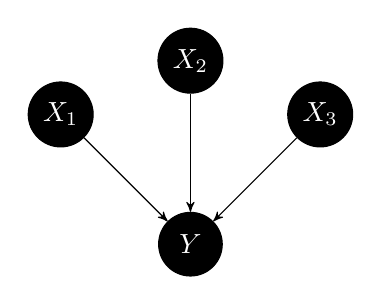
\begin{tikzpicture}
		\node[obs] (Y) {$Y$} ;
		\node[obs, above right=of Y] (X2) {$X_3$} edge[->] (Y) ;
		\node[obs, above =of Y] (X1) {$X_2$} edge[->] (Y) ;
		\node[obs, above left=of Y] (X0) {$X_1$} edge[->] (Y) ;
	\end{tikzpicture}
			\label{fig:pc_not_markov_gt}
		}
		\hspace{1.5cm}
		\subfloat[Intermediate skeleton that PC finds after conducting all marginal independence tests.]{
			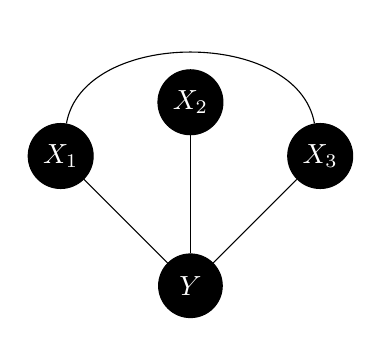
\begin{tikzpicture}
		\node[obs] (Y) {$Y$} ;
		\node[obs, above right=of Y] (X2) {$X_3$} edge[-] (Y) ;
		\node[obs, above =of Y] (X1) {$X_2$} edge[-] (Y) ;
		\node[obs, above left=of Y] (X0) {$X_1$} edge[-] (Y) ;
        \draw (X0) edge[-, bend left=80] (X2);
	\end{tikzpicture}
			\label{fig:pc_not_markov_intermediate}
		}
		\hspace{1.5cm}
		\subfloat[Final skeleton that PC finds before orienting the edges.]{
			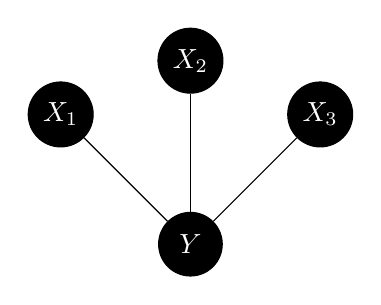
\begin{tikzpicture}
		\node[obs] (Y) {$Y$} ;
		\node[obs, above right=of Y] (X2) {$X_3$} edge[-] (Y) ;
		\node[obs, above =of Y] (X1) {$X_2$} edge[-] (Y) ;
		\node[obs, above left=of Y] (X0) {$X_1$} edge[-] (Y) ;
	\end{tikzpicture}
			\label{fig:pc_not_markov_undirected}
		}
		\caption{This example illustrates how the PC algorithm arrives at a graph that contradicts a dependence statement used as input to the algorithm.}
		\label{fig:pc_not_markov}
	\end{figure}
\end{example}

    \section{Experimental Details}
\label{sec:experiment_details}
The source code for the experiments can be found under \href{https://github.com/PhilippFaller/RedundancyInGraphDiscovery}{\url{https://github.com/PhilippFaller/RedundancyInGraphDiscovery}}. 
\todo{Don't forget to change this before resubmission.}


For the experiment in \cref{fig:p_values_redundant} we first generate a DAG with four nodes according to an Erdös-Rényi model with edge probability $1/2$.
We then uniformly draw coefficients for a linear structural equation model \citep{pearl2009causality} from $(-1, -0.1] \cup [0.1, 1)$.
For each variable we add Gaussian noise with zero mean and unit variance.
We generate 300 samples for each dataset.
Then, we randomly permute a list containing all triplets in $\CI(\bV)$, where $\bV$ is the set of nodes.
For every triplet $(X, Y, \bZ)$ in this list we conduct a Fisher $Z$ test for independence, implemented in \texttt{causal-learn} \citep{zheng2024causal}.
We also check with the \texttt{Z3} SMT solver \citep{z3} whether the result of $\CI(X, Y\mid \bZ)$ follows from the previously conducted tests (with $\alpha$-threshold $0.01$) via Graphoid axioms.
If so, we add the $p$-value of the test to either the list of implied dependences or independences, respectively to the Graphoid implication.
We repeat the same experiment 16 times and keep adding the $p$-values to the same lists.
The plot shows these two lists of $p$-values and $\alpha$.

For the experiment in \cref{fig:graphically_redundant_two_datasets} we generate two kinds of dataset, one generated by a DAG and the other one by an undirected graphical model.
The ground truth graphs can be seen in \cref{fig:ground_truth_two_datasets}.
All variables are binary.
For the DAG, we draw coefficients for the conditional distributions of each variable given all possible values of their parents.
We then recursively sample the values along the topological ordering of the graph, starting from $W$.
We drew $P(X=1 \ |\  W=0),\, P(Y=1 \ | \  W=0),\, P(Z=1\ | \  X=0, Y=0)$ and $P(Z=1\ |\  X=1, Y=1)$ uniformly from $[0.3, 0.7)$ and then set
\begin{align*}
    P(X=1 \mid W=1) &= 1-P(X=1 \mid W=0)\\
    P(Y=1 \mid W=1) &= 1-P(Y=1 \mid W=0)\\
    P(Z=1\mid X=0, Y=1) &= 1- P(Z=1\mid X=0, Y=0)\\
    P(Z=1\mid X=1, Y=0) &= 1- P(Z=1\mid X=1, Y=1).
\end{align*}
For the undirected model, we used the \texttt{pgmpy} package \citep{ankan2024pgmpy}.
For each edge $X-Y$ in the graph, we add a factor $\phi$ to a factor graph model, where we pick the value $\phi(X=0, Y=0)$ and $\phi(X=1, Y=1)$ uniformly from $[0.1, 0.3)$ and set 
\begin{align*}
\phi(X=0, Y=1) &= 1 - \phi(X=0, Y=0) \\
\phi(X=1, Y=0) &= 1- \phi(X=1, Y=1).
\end{align*}
We then draw the distribution using Gibbs sampling with the default parameters of \texttt{pgmpy}.
Note, that neither of the graphs' independence models is Markovian and faithful to the other.
For each dataset we generated 300 samples.

We then use the tests described in \cref{prop:markov_network_markovian,prop:protocol_graph_markovian} to construct an undirected graphical model and a DAG on each dataset, where we used the $\chi^2$-test implemented in \texttt{causal-learn} with $\alpha$-threshold $0.01$.

Finally, we identify purely graphically redundant tests using \cref{prop:sufficient_cond_non_graphoid}.
We conduct these tests and report the fraction of CI-tests, where the graphical implication contradicts the empirical test result. After conducting a test, we add it to the set of previously conducted tests.
We repeated the experiment 1000 times.

\begin{figure}[htp]
	\centering
    \subfloat[Ground truth for the DAG datasets in \cref{fig:graphically_redundant_two_datasets}.]{
	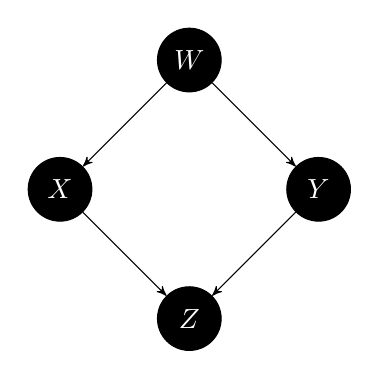
\begin{tikzpicture}
		\node[obs] (W) {$W$} ;
		\node[obs, below left=of W] (X) {$X$} edge[<-] (W) ;
		\node[obs, below right =of W] (Y) {$Y$} edge[<-] (W) ;
		\node[obs, below right=of X] (Z) {$Z$} edge[<-] (X) ;
		\draw (Y) edge[->] (Z);
		
	\end{tikzpicture}
    }\hspace{2cm}
    \subfloat[Ground truth for the undirected graph datasets in \cref{fig:graphically_redundant_two_datasets}.]{
    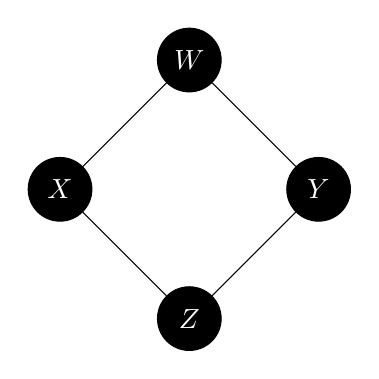
\begin{tikzpicture}
		\node[obs] (W) {$W$} ;
		\node[obs, below left=of W] (X) {$X$} edge[-] (W) ;
		\node[obs, below right =of W] (Y) {$Y$} edge[-] (W) ;
		\node[obs, below right=of X] (Z) {$Z$} edge[-] (X) ;
		\draw (Y) edge[-] (Z);
		
	\end{tikzpicture}
    }
	\caption{Ground truth graphs for the experiment in \cref{fig:graphically_redundant_two_datasets}.}
	\label{fig:ground_truth_two_datasets}
\end{figure}

For \cref{fig:tree_discovery} we first pick a random spanning tree with four nodes.
To this end we initialise a matrix with uniformly distributed numbers from $[0, 1)$, interpret it as adjacency matrix of a weighted graph and find a maximum weight spanning tree using Kruskal's algorithm.
We then pick a node as root uniformly at random  and orient all edges away from the root in a depth-first search to get a Markov-equivalent DAG.
Then we can recursively draw samples from this graph.
As before, we uniformly pick coefficients for a linear structural causal model from $(-1, -0.1] \cup [0.1, 1)$ and draw noise from a standard normal distribution.
For each dataset we generate 1000 samples.

To find the underlying tree under the MMD assumption, we conduct all CI-tests in the set $S$ from \cref{prop:error_correction_trees} using the Fisher $Z$ test from \texttt{causal-learn} with $\alpha$-threshold $0.01$.
We calculate the Markov-distance w.r.t. $S$ for all possible spanning trees over the nodes.

As a baseline we consider a simplified version of the PC algorithm.
This way, we only use tests of the same conditioning set size and can rule out that the difference is due to the statistical condition of the problem.
First, we skip the initial phase, where PC would conduct all marginal independence tests, as in a spanning tree all nodes are dependent anyway.
We then proceed with the tests with a single conditioning variable as usual.
Since in the limit of infinite data, these tests are already sufficient to identify the graph, we do not consider larger conditioning sets.
Further, we stop once the current graph is a tree, as any further CI-tests could only violate the spanning property.

For each of the resulting graphs we calculate the structural Hamming distance \citep{tsamardinos2006max}, i.e. the number of differing edges, to the ground truth graph and also record for each dataset the difference between the two SHD scores.
We repeat the experiment for 1000 datasets.

All experiments were run on an Apple M3 Pro processor with 18 GB RAM. The experiment for \cref{fig:p_values_redundant} took roughly a day while the other experiments finished in a couple of minutes.
\end{document}

